\documentclass{article}\usepackage[]{graphicx}\usepackage[]{xcolor}
% maxwidth is the original width if it is less than linewidth
% otherwise use linewidth (to make sure the graphics do not exceed the margin)
\makeatletter
\def\maxwidth{ %
  \ifdim\Gin@nat@width>\linewidth
    \linewidth
  \else
    \Gin@nat@width
  \fi
}
\makeatother

\definecolor{fgcolor}{rgb}{0.345, 0.345, 0.345}
\newcommand{\hlnum}[1]{\textcolor[rgb]{0.686,0.059,0.569}{#1}}%
\newcommand{\hlsng}[1]{\textcolor[rgb]{0.192,0.494,0.8}{#1}}%
\newcommand{\hlcom}[1]{\textcolor[rgb]{0.678,0.584,0.686}{\textit{#1}}}%
\newcommand{\hlopt}[1]{\textcolor[rgb]{0,0,0}{#1}}%
\newcommand{\hldef}[1]{\textcolor[rgb]{0.345,0.345,0.345}{#1}}%
\newcommand{\hlkwa}[1]{\textcolor[rgb]{0.161,0.373,0.58}{\textbf{#1}}}%
\newcommand{\hlkwb}[1]{\textcolor[rgb]{0.69,0.353,0.396}{#1}}%
\newcommand{\hlkwc}[1]{\textcolor[rgb]{0.333,0.667,0.333}{#1}}%
\newcommand{\hlkwd}[1]{\textcolor[rgb]{0.737,0.353,0.396}{\textbf{#1}}}%
\let\hlipl\hlkwb

\usepackage{framed}
\makeatletter
\newenvironment{kframe}{%
 \def\at@end@of@kframe{}%
 \ifinner\ifhmode%
  \def\at@end@of@kframe{\end{minipage}}%
  \begin{minipage}{\columnwidth}%
 \fi\fi%
 \def\FrameCommand##1{\hskip\@totalleftmargin \hskip-\fboxsep
 \colorbox{shadecolor}{##1}\hskip-\fboxsep
     % There is no \\@totalrightmargin, so:
     \hskip-\linewidth \hskip-\@totalleftmargin \hskip\columnwidth}%
 \MakeFramed {\advance\hsize-\width
   \@totalleftmargin\z@ \linewidth\hsize
   \@setminipage}}%
 {\par\unskip\endMakeFramed%
 \at@end@of@kframe}
\makeatother

\definecolor{shadecolor}{rgb}{.97, .97, .97}
\definecolor{messagecolor}{rgb}{0, 0, 0}
\definecolor{warningcolor}{rgb}{1, 0, 1}
\definecolor{errorcolor}{rgb}{1, 0, 0}
\newenvironment{knitrout}{}{} % an empty environment to be redefined in TeX

\usepackage{alltt}
\usepackage{graphicx} 
\usepackage{geometry} 
\usepackage{listings}
\usepackage{xcolor}
\usepackage{fancyhdr}
\usepackage{natbib}

\definecolor{codebg}{rgb}{0.95, 0.95, 0.95}
\lstset{language=R,
backgroundcolor=\color{codebg},
    basicstyle=\ttfamily,
    keywordstyle=\color{blue},
    stringstyle=\color{orange},
    commentstyle=\color{gray},
    showstringspaces=false,
    frame=single,
    breaklines=true,
    postbreak=\mbox{\textcolor{red}{$\hookrightarrow$}\space}
}

\geometry{
    top=2cm,
    bottom=2cm,
    left=2cm,
    right=2cm,
}
\pagestyle{fancy}
\fancyhf{}
\fancyhead[L]{Nayan Subedi}
\fancyhead[R]{Student.I.D 23140735}
\fancyfoot[L]{\includegraphics[width=0.05\textwidth]{logo.png}}
\fancyfoot[C]{}
\fancyfoot[R]{\thepage}
\IfFileExists{upquote.sty}{\usepackage{upquote}}{}
\begin{document}


\begin{figure}[t]
    \centering
    \includegraphics[width=0.3\textwidth]{logo.png}
\end{figure}

\title{World Economic Indicators}
\author{Nayan Subedi\\ Student I.D 23140735 \\ CMP5352 Data Visualisation\\ Words Count: 4993}
\date{\today}
\maketitle

\newpage

\begin{abstract}
This paper explores socio-economic and demographic trends across various regions and income groups from 2000 to 2018 using World Bank data. The analysis focuses on key indicators like unemployment rates, life expectancy, GDP per capita, infant mortality rate, birth and death rates, electric power consumption, internet usage, and population density. Findings highlight significant global progress in reducing infant mortality and improving life expectancy, particularly in regions with increasing GDP per capita. However, disparities persist across income groups and regions, emphasizing the influence of factors beyond wealth on overall well-being.
\end{abstract}

\textbf\textit{Keywords:}\textit{ World Bank data, life expectancy, GDP per capita, infant mortality rate, birth rate, death rate, internet usage, population density, electric power consumption, regional disparities, global development.}

\newpage
\tableofcontents

\newpage
\listoffigures
\newpage

\section{Introduction}
Using data from the World Bank, this report explores the complex relationships between economic and demographic changes globally from 2000 to 2018. We seek to identify the broad patterns in global development by looking at important metrics such as life expectancy, GDP per capita, infant mortality rates, birth and death rates, internet usage, electric power consumption, and population density. We investigate regional disparities between regions such as Europe and Central Asia, East Asia and Pacific, and Sub-Saharan Africa. We also examine how differences in income groups affect social indices by contrasting the patterns observed in high- and low-income countries.The goal of report is to provide a comprehensive and insightful image of the complex dynamics of global development by means of data visualization, highlighting both advancements and continuing difficulties. The purpose of this report is to give scholars, politicians, and anybody else who is interested in learning more about the dynamics of global change and the factors influencing the world's future useful insights.

\newpage


\section{Aim and Objective of the Report}

The report aims to explore the socio-economic and demographic trends that differ across regions and countries in the time period from 2000 to 2018. The analysis seeks to elucidate trends in some of the key crude measures (unemployment rate, life expectancy, GDP per capita, infant mortality rate, childbirth and fertility rates, death rate, electric power consumption, Internet usage, etc.) over time and as a function of region and income class.

\subsection{Objective of the Report}

I have drafted a number of non-trivial questions and visualized the questions to make these trends and relationships quite clear in the analysis.

\subsection{Non-Trivial Questions}

\textbf{Trend Analysis and Comparisons}

\begin{itemize}
    \item How have unemployment rates evolved across different regions and income groups?
    \item Does the relationship between life expectancy and GDP per capita vary across regions and income groups?
    \item What is the trend of Life Expectancy in regions with different population Density?
    \item How has the infant mortality rate changed over time in different regions?
    \item Are there differences in the rate of change in birth rates between regions or income groups?
    \item Is the relationship between income group and death rate consistent across regions?
    \item{How do birth rates and infant mortality rates vary across different regions? Are there significant differences between regions?}
\end{itemize}

\textbf{Correlation and Relationships}

\begin{itemize}
    \item Is there a strong correlation between internet usage and GDP per capita?
    \item What are the correlations among various socio-economic variables in the dataset?
\end{itemize}

\newpage

\section{Loading Libraries}

\begin{lstlisting}
library(ggplot2)
library(dplyr)
library(tidyverse)
library(reshape2)
library(RColorBrewer)
library(rworldmap)
library(viridis)
\end{lstlisting}
These packages are used for complete data visualization in the project. They are used to create aesthetically pleasing plots, perform data manipulation, and represent geographical data.





\subsection{Data Preperation}
\begin{lstlisting}
wb_data <- read.csv("WorldBank.csv")
\end{lstlisting}

The data "WorldBank.csv" is loaded into the R.

\subsection{Data exploration}
\begin{lstlisting}
str(wb_data)
summary(wb_data)
\end{lstlisting}

The str() and summary() functions  are used to display the structure and a statistical summary of a data object respectively.

\section{Data Wrangling and Cleaning}
Preparing data for analysis involves crucial steps known as data wrangling and cleaning. Data wrangling is the process of taking raw data and making it more usable. This includes gathering data from different sources, understanding its structure and quality, fixing any errors or inconsistencies, converting it into the required format, adding new information to enhance it, and ensuring the changes maintain accuracy. Data cleaning, a part of data wrangling, specifically aims to improve the quality of the data by dealing with missing values, eliminating duplicates, correcting mistakes, standardizing formats, filtering out unusual values, converting data types, and normalizing the data. These steps ensure that the data is accurate and complete, leading to more reliable and meaningful analysis results.
The report contains a few step of data wrangling and cleaning practices.

\subsection{Data Cleaning}
\subsubsection{Renaming column name for better readability}
\begin{lstlisting}
names(wb_data) <- c(
  "Country", "Country_Code", "Region", "Income_Group", "Year", 
  "Birth_Rate", "Death_Rate", 
  "Electric_Power_Consumption_per_Capita", "GDP", "GDP_per_Capita", 
  "Internet_Users_Percentage", "Infant_Mortality_Rate", 
  "Life_Expectancy", "Population_Density", 
  "Unemployment_Rate")
\end{lstlisting}

A  standard naming convention is used in this  projects had facilitate better data management and visualization.

\newpage
\subsubsection{Missing Values}
\begin{lstlisting}
sum(is.na(wb_data))
\end{lstlisting}
\begin{knitrout}
\definecolor{shadecolor}{rgb}{0.969, 0.969, 0.969}\color{fgcolor}\begin{kframe}
\begin{verbatim}
## [1] 33356
\end{verbatim}
\end{kframe}
\end{knitrout}
When I check for null values in my dataset and find 33,356 missing values, this total represents the number of missing values across all rows and columns in the entire dataset. This includes data 1970-2018.

\subsubsection{Filtering the dataset}
\begin{lstlisting}
world_bank_data <- wb_data %>% 
  filter(Year >= 2000 & Year <= 2018)
  sum(is.na(world_bank_data))
\end{lstlisting}
\begin{knitrout}
\definecolor{shadecolor}{rgb}{0.969, 0.969, 0.969}\color{fgcolor}\begin{kframe}
\begin{verbatim}
## [1] 4885
\end{verbatim}
\end{kframe}
\end{knitrout}
when I filter the dataset to only include data from the years 2000 to 2018. I am narrowing down the dataset to a specific time range. By doing so, the number of rows in the filtered dataset is reduced because it excludes data from years outside of this range. Consequently, the number of missing values in the filtered dataset drops to 4,885.

\section{Visualization}
\subsection{Trend Analysis and Comparisons}

\subsubsection{unemployment rates across different regions and income groups}
\begin{lstlisting}
unemployment_data <- world_bank_data %>%
  select(Year, Region, Income_Group, Unemployment_Rate) %>%
  na.omit() %>%
  group_by(Year, Region, Income_Group) %>%
  summarise(Average_Unemployment = mean(Unemployment_Rate))

ggplot(Unemployment_data, aes(x = Year, y = Average_Unemployment, color = Income_Group)) +
  geom_line(size = 1.2) + 
  facet_wrap(~Region, scales = "free_y", ncol = 3) + 
  labs(title = "Trend in Unemployment Rates by Income Group and Region",
       x = "Year",
       y = "Unemployment (% of total labor force)",
       color = "Income Group") +
  theme_minimal() +
  theme(
    plot.title = element_text(size = 18, face = "bold", hjust = 0.5), 
    axis.title = element_text(size = 14), 
    axis.text = element_text(size = 12), 
    legend.title = element_text(size = 14), 
    legend.text = element_text(size = 12), 
    strip.text = element_text(size = 14, face = "bold"), 
    panel.grid.major = element_line(color = "grey80", linetype = "dashed", size = 0.5),
    panel.grid.minor = element_blank() 
  ) 

\end{lstlisting}
\begin{figure}[h!]
\centering
\begin{knitrout}
\definecolor{shadecolor}{rgb}{0.969, 0.969, 0.969}\color{fgcolor}
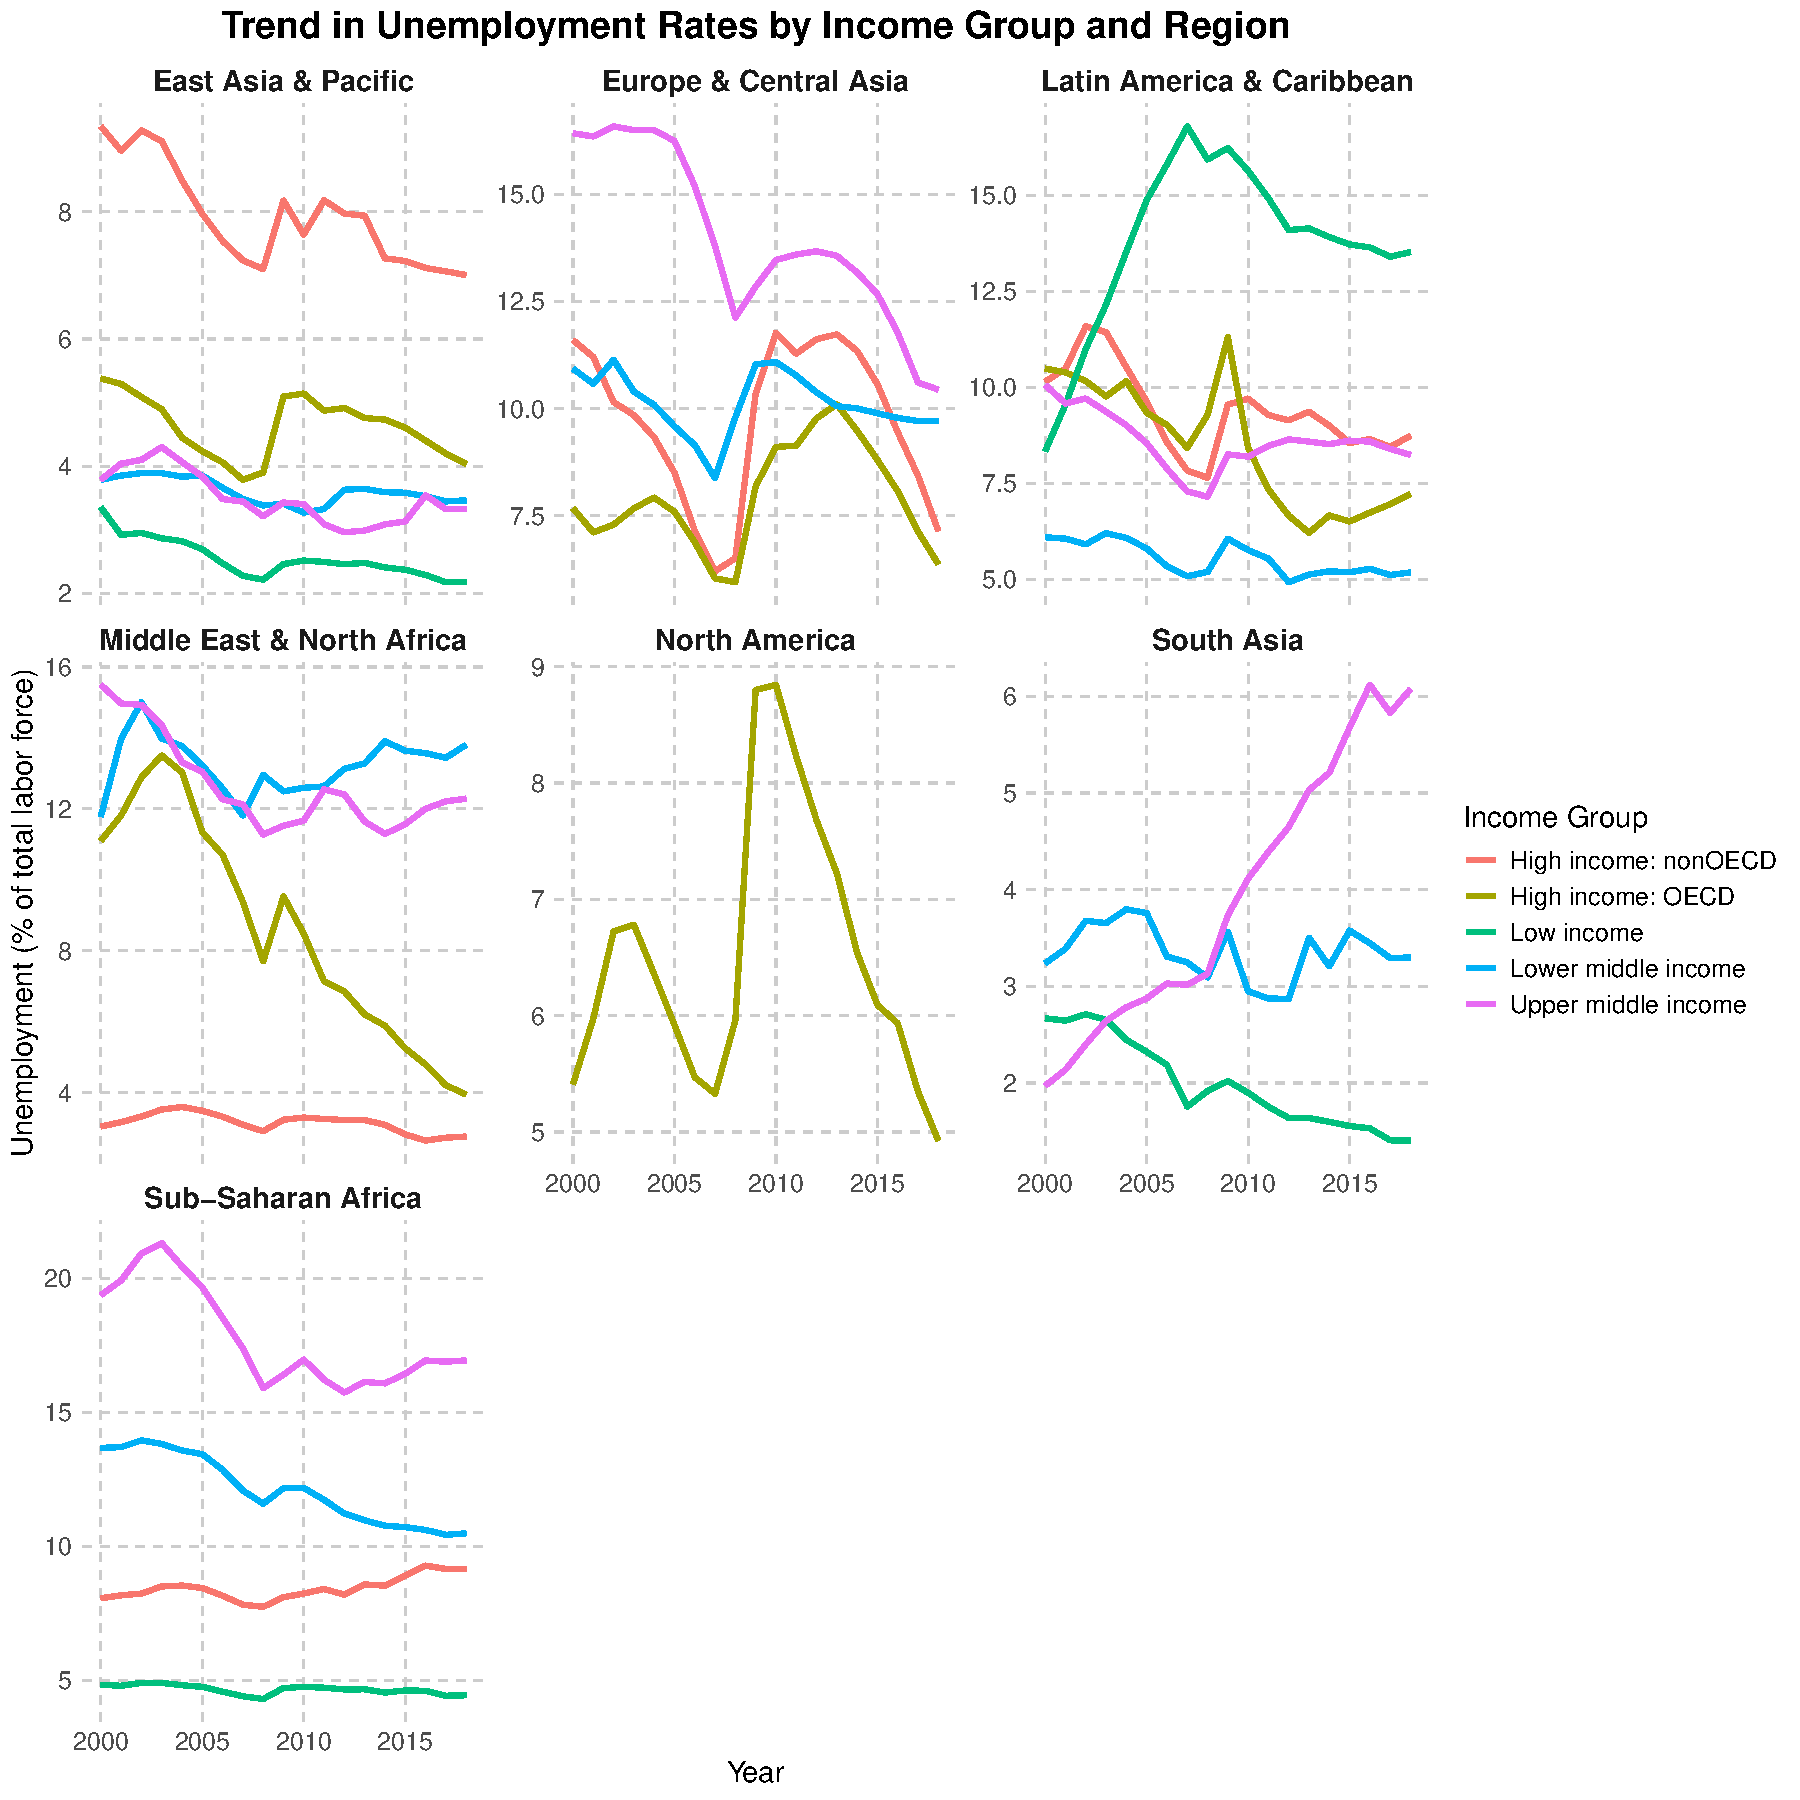
\includegraphics[width=\maxwidth]{figure/unnamed-chunk-6-1} 
\end{knitrout}
\caption{Trend in Unemployment Rates by Income Group and Region}
\label{fig}
\end{figure}
This plot shows the trend  of unemployment rates by type of income and different regions over 2000-2018.The plot is divided into six plots, corresponding to the  regions: East Asia and Pacific , Europe and Central Asia , Latin America and Caribbean , Middle East and North Africa , North America  and Sub-Saharan Africa.\hfill \break

The unemployment rates for five income groups high income: nonOECD; high income: OECD; low income; lower middle income; and upper middle income are displayed in horizontal subplots. The Unemployment Rate is plotted in percentage of the Labor Force.\hfill \break

The plot shows that unemployment rates have generally trended downwards in most regions, with the exception of Sub-Saharan Africa and Latin America and Caribbean. There are some notable key findings from the plot:

\textbf{Regional Trends}
\begin{itemize}

\item{Europe and Central Asia experienced the peaks in unemployment, particularly after the 2008. Upper middle countries in this region were hit hard, but recovered relatively well.}

\item{Latin America and Caribbean showed a fluctuating but generally improving trend in unemployment, with Low Income countries consistently having the highest rates in the region.}

\item{East Asia and Pacific has maintained relatively stable unemployment rates throughout the period, with gradual decreases in most income groups.}

\item{Middle East and North Africa high-income non-OECD countries faced the least unemployment compared to other income groups in this region.}

\item{North America witnessed a sharp spike in unemployment around 2008-2010 (likely due to the financial crisis), followed by a steady decline.}

\item{South Asia eperienced a consistent decline in unemployment for Low Income, while Upper middle income is constantly increasing. }

\item{Sub-Saharan Africa had the unemployment rate remained constant throughout the years.}
\end{itemize}

\textbf{Overall Observations}

The unemployment rates are generally higher in the low and lower-middle income groups. There is a clear trend of lower unemployment rates in the high-income groups, particularly in high-income OECD countries. The plot helps to visualize the relationship between income group, unemployment rate, and region.

\subsubsection{Life expectancy across different regions and income groups}
\begin{lstlisting}
life_gdp_data <- world_bank_data %>%
  select(Life_Expectancy, GDP_per_Capita, Income_Group, Region) %>%
  na.omit()

options(scipen = 20)
ggplot(life_gdp_data, aes(x = GDP_per_Capita, y = Life_Expectancy, color = Income_Group)) +
  geom_point(alpha = 0.7, size = 3) + 
  facet_wrap(~Region, ncol = 3) +  
  labs(title = "Life Expectancy and GDP per Capita by Region and Income Group ",
       x = "GDP per Capita (Current US$)",
       y = "Life Expectancy (Years)",
       color = "Income Group") +
  theme_bw() +  
  theme(
    axis.text = element_text(size = 10),
    axis.title = element_text(size = 12, face = "bold"),
    plot.title = element_text(size = 16, face = "bold", hjust = 0.5),
    legend.position = "bottom", 
    legend.text = element_text(size = 10),
    legend.title = element_text(size = 12, face = "bold"),
    strip.text = element_text(size = 12, face = "bold"),
    panel.grid.major = element_line(color = "gray90", linetype = "dashed"),
    panel.grid.minor = element_line(color = "gray95", linetype = "dashed")
  ) +
  scale_x_log10()  
\newpage

\end{lstlisting}
\begin{figure}[h!]
\centering
\begin{knitrout}
\definecolor{shadecolor}{rgb}{0.969, 0.969, 0.969}\color{fgcolor}
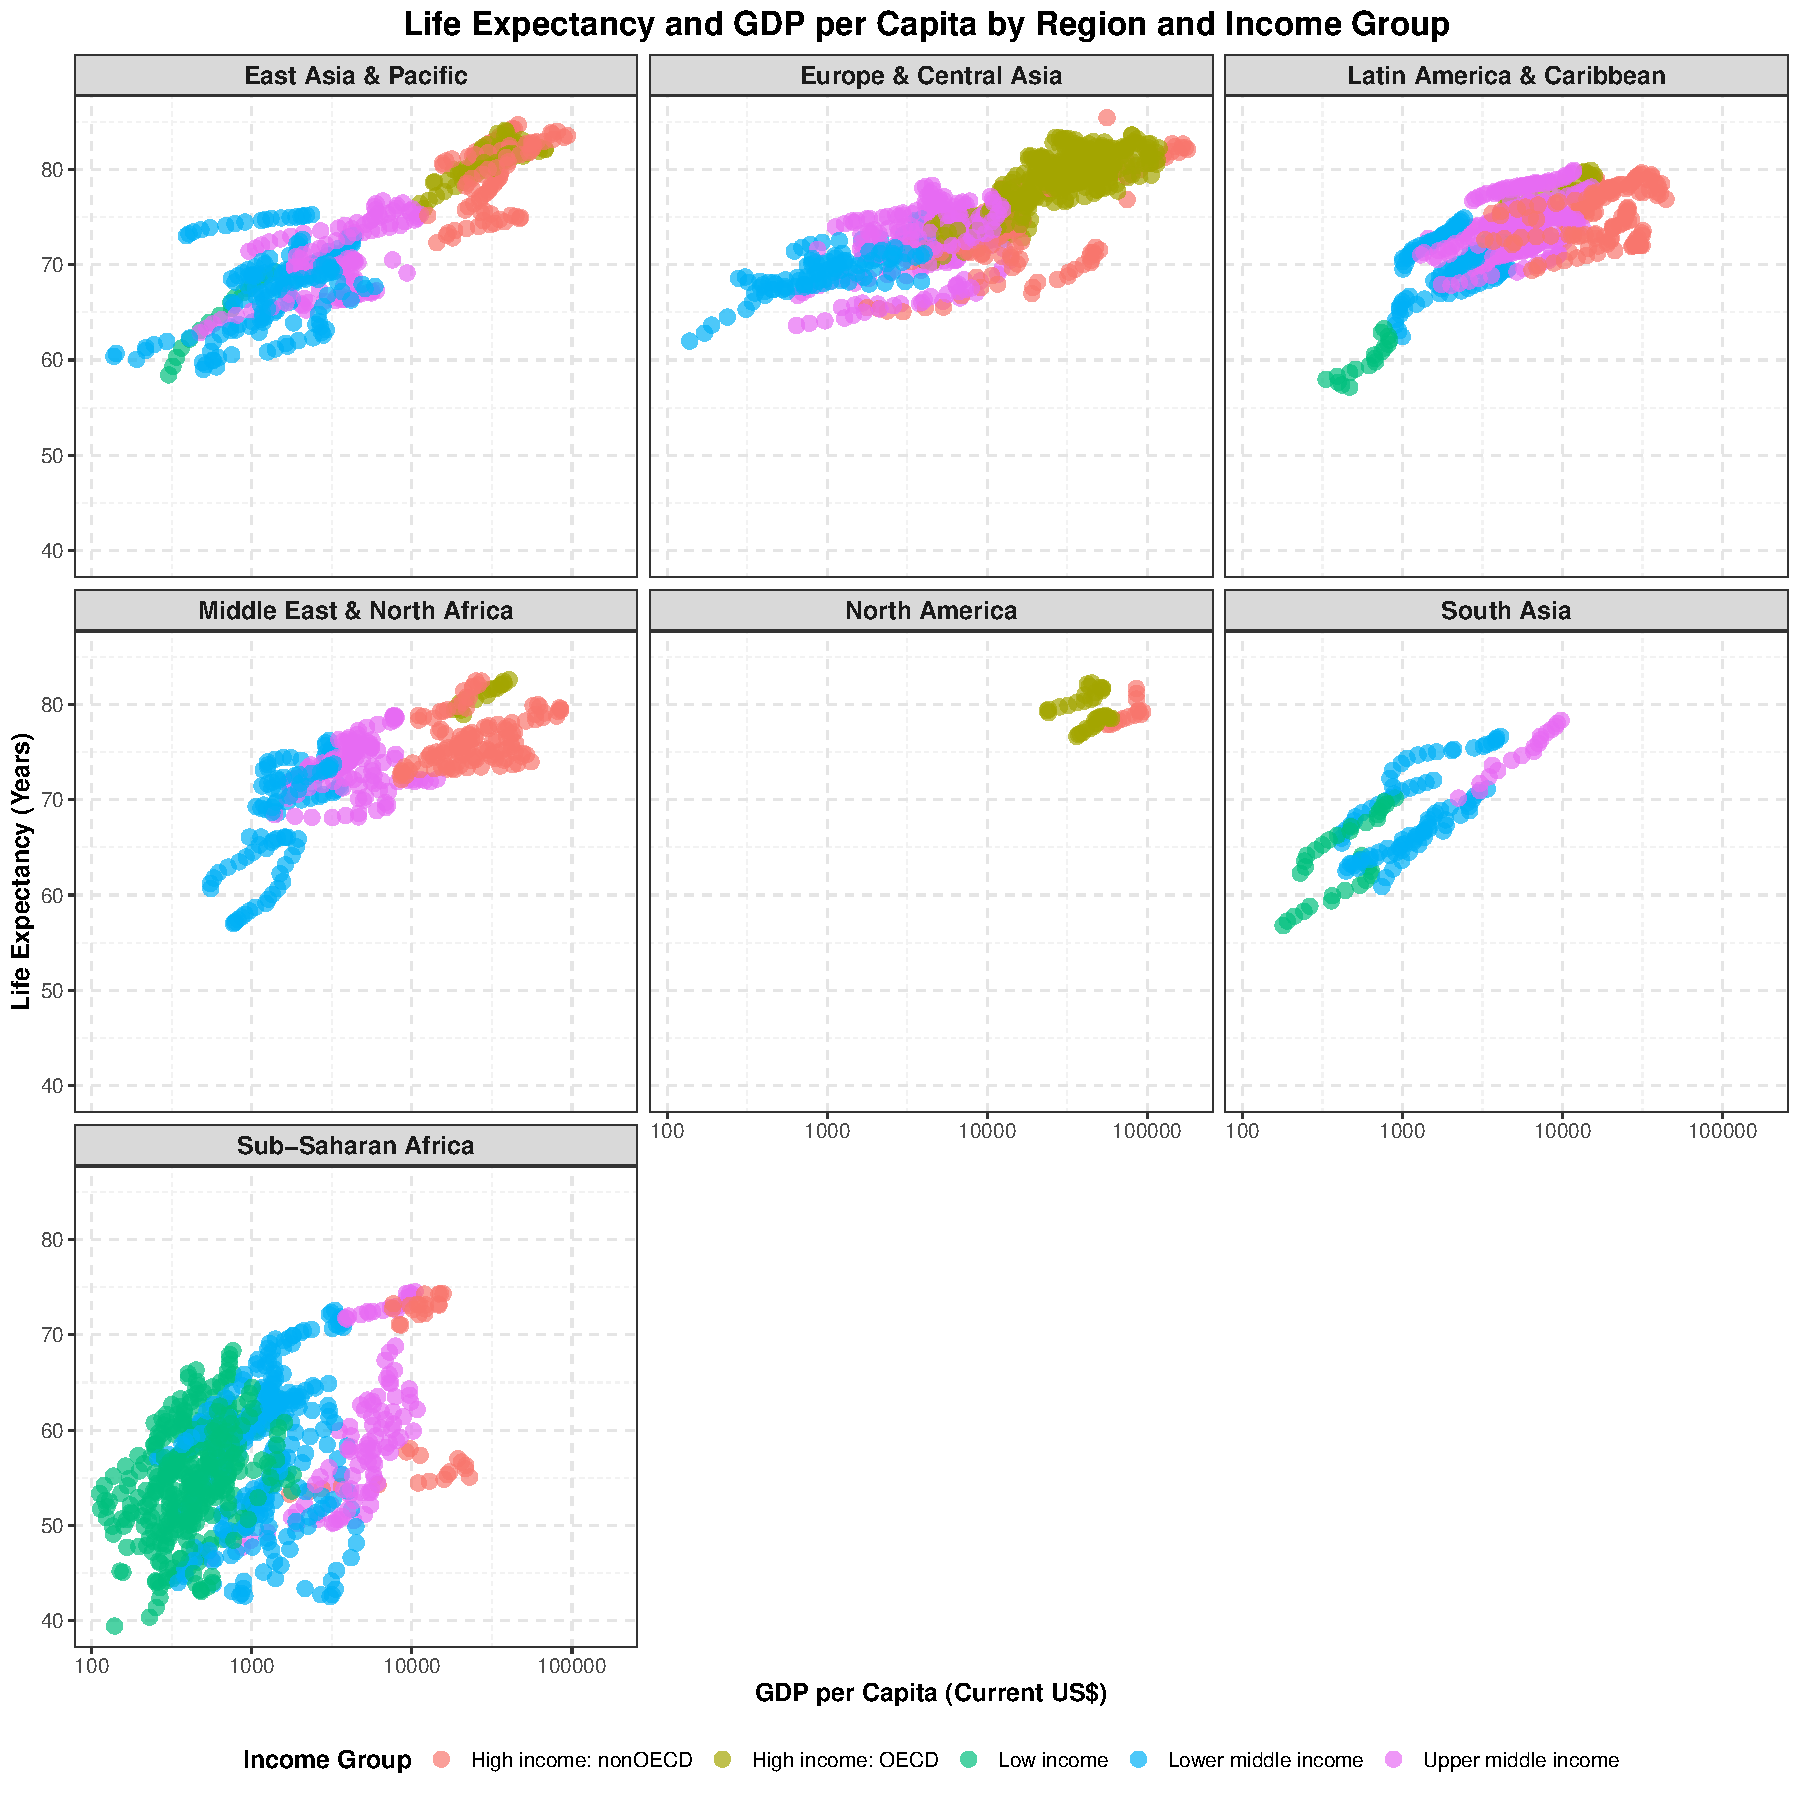
\includegraphics[width=\maxwidth]{figure/unnamed-chunk-7-1} 
\end{knitrout}
\caption{Trend in Life Expectancy by Income Group and Region}
\label{fig}
\end{figure}

The plot shows that life expectancy have generally trended upwards in most regions, with the exception ofsome income groups. There are some notable key findings from the plot:

\textbf{General Trend}
\begin{itemize}

\item{There's a clear positive correlation between GDP per capita and life expectancy. This means wealthier countries and income groups tend to have longer lifespans, reflecting their better GDP per Capita, better healthcare, nutrition, sanitation, and living conditions.}
\end{itemize}

\textbf{Regional Trend}
\begin{itemize}
\item{East Asia  and Pacific and Europe and Central Asia showed a tight clustering along the upward trend, indicating a strong link between high GDP per Capita and life expectancy.}

\item{Latin America and Caribbean, Middle East and North Africa, South Asia  regions illustrates a wider spread of data points. While the upward trend is still present, it suggests greater variation within each region – some countries achieve higher life expectancies at lower GDP levels compared to others.}

\item{Sub-Saharan Africa region, while also showing a positive correlation, has a lower overall life expectancy compared to other regions at similar GDP levels. This points to factors beyond just wealth affecting lifespan, such as access to healthcare, disease burden, and social determinants of health.}
\end{itemize}


\textbf{Overall Observations}

The plot highlights the complex relationship between region, GDP per Capita, and Income Groups.Longer life expectancies are often correlated with higher GDP per capita; nevertheless, regional differences and income group differences highlight the impact of additional important factors on a country's well-being.


\subsubsection{Life Expectancy by Population Density and Region}
\begin{lstlisting}
ggplot(world_bank_data, aes(x = Life_Expectancy, y = GDP_per_Capita, size = Population_Density, color = Region)) +
  geom_point(alpha = 0.7, shape = 20, stroke = 0.75) +  
  scale_y_log10(labels = scales::comma) + 
  scale_size_continuous(range = c(2, 10), name = "Population Density\n(people per sq. km)") +  
  scale_color_brewer(palette = "Set1") +  
  labs(title = "Life Expectancy by Population Density and Region",  
       x = "Life Expectancy (Years)",
       y = "GDP per Capita") + 
  theme_bw() +  
  theme(
    panel.grid.major = element_line(color = "grey80", size = 0.2),
    panel.grid.minor = element_line(color = "grey90", size = 0.1),
    axis.title = element_text(face = "bold", size = 12),
    axis.text = element_text(size = 10),
    plot.title = element_text(face = "bold", size = 14),
    legend.title = element_text(face = "bold", size = 10),
    legend.text = element_text(size = 9)
  ) +
  guides(color = guide_legend(title = "Region", override.aes = list(size = 5)))  
\end{lstlisting}
\newpage
\begin{figure}[h!]
\centering
\begin{knitrout}
\definecolor{shadecolor}{rgb}{0.969, 0.969, 0.969}\color{fgcolor}
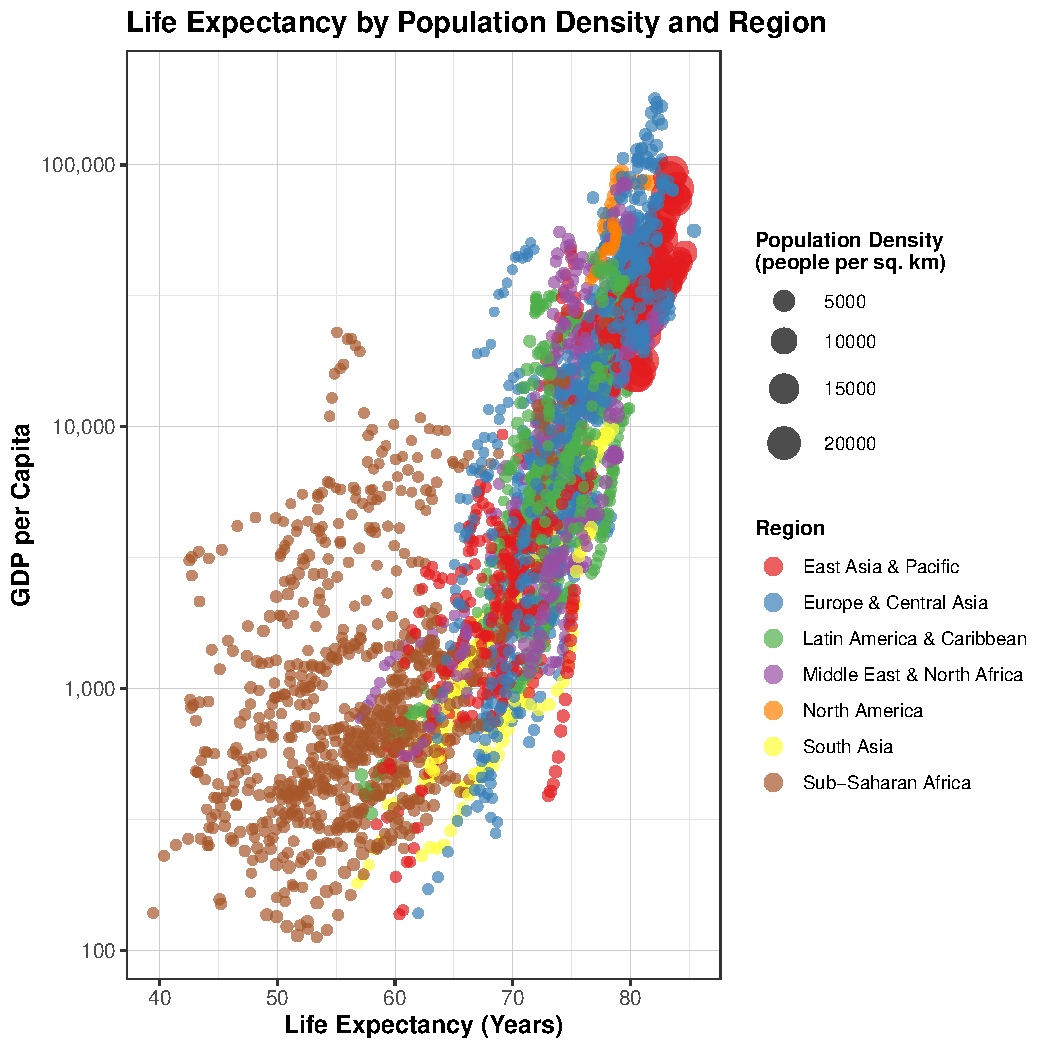
\includegraphics[width=\maxwidth]{figure/unnamed-chunk-8-1} 
\end{knitrout}
\caption{Trend in Life Expectancy by Population Density and Region}
\label{fig}
\end{figure}

The trend observed in regions with high population density shows that as life expectancy increases, the population density also tends to increase. However, there is a wide variation within each region

\textbf{Regional  Trend}
\begin{itemize}

\item{East Asia and Pacific: The life expectancy in this region varies significantly, ranging from about 50 to 90 years according to Countries GDP per capita. There are large variations in population density, with some regions having high densities (over 20.000 people per square kilometer) and others having lower densities .Overall, life expectancy and population density appear to be positively correlated.}

\item{Europe and Central Asia: These regions typically have high life expectancies.Although there are differences in population density, most places are between moderate and high densities.The trend indicates that a higher population density is linked to a longer life expectancy.}

\item{Latin America and Caribbean: This region have average lifespan range between 60 and 80 years.There are large differences in population density, with some areas having low and others having moderate densities.Here, there is a a less strong relationship between population density and life expectancy.}

\item{Middle East and North Africa:The average lifespan ranges from 60 to 80 years. Although it varies, most places have a modest population density. In this area, the association between population density and life expectancy is less clear.}

\item{North America : The average lifespan is quite high. In Certain places, population density is almost constant to 10,000 people per sq km .High in GDP per capita  indicates that this region has  higher population density is linked to a longer life expectancy .}

\item{South Asia: The average lifespan is between 50 and 75 years. In Certain places, population density is very high (over 20,000people per sq km).Connection  between Population density and life expectancy appear to be slightly less likely due to its weak GDP per Capita.}


\end{itemize}


\textbf{Overall Observations}
We frequently observe higher population densities in areas with longer life expectancies.
There are, however, outliers in every location, highlighting the impact of additional variables (such the availability of healthcare, socioeconomic status, and urbanization) on life expectancy.

\subsubsection{Infant Mortality Rate by Region }
\begin{lstlisting}
infant_mortality_data <- world_bank_data %>%
  select(Year, Region, Infant_Mortality_Rate) %>%
  na.omit() %>%
  group_by(Year, Region) %>%
  summarise(Average_Infant_Mortality = mean(Infant_Mortality_Rate))

ggplot(infant_mortality_data, aes(x = Year, y = Average_Infant_Mortality, color = Region)) +
  geom_line(size = 1) +  
  labs(title = "Trend in Infant Mortality Rate by Region",
       x = "Year",
       y = "Infant Mortality Rate (per 1,000 live births)",
       color = "Region") +
  theme_minimal() +
  
  scale_color_brewer(palette = "Set1") +  
  theme(
    plot.title = element_text(size = 16, face = "bold"),  
    axis.title = element_text(size = 12),                
    legend.title = element_text(size = 12),              
    panel.grid.major = element_line(color = "grey90", linetype = "dashed"),   
    panel.grid.minor = element_blank()                   
  ) 

\end{lstlisting}
\newpage
\begin{figure}[h!]
\centering
\begin{knitrout}
\definecolor{shadecolor}{rgb}{0.969, 0.969, 0.969}\color{fgcolor}
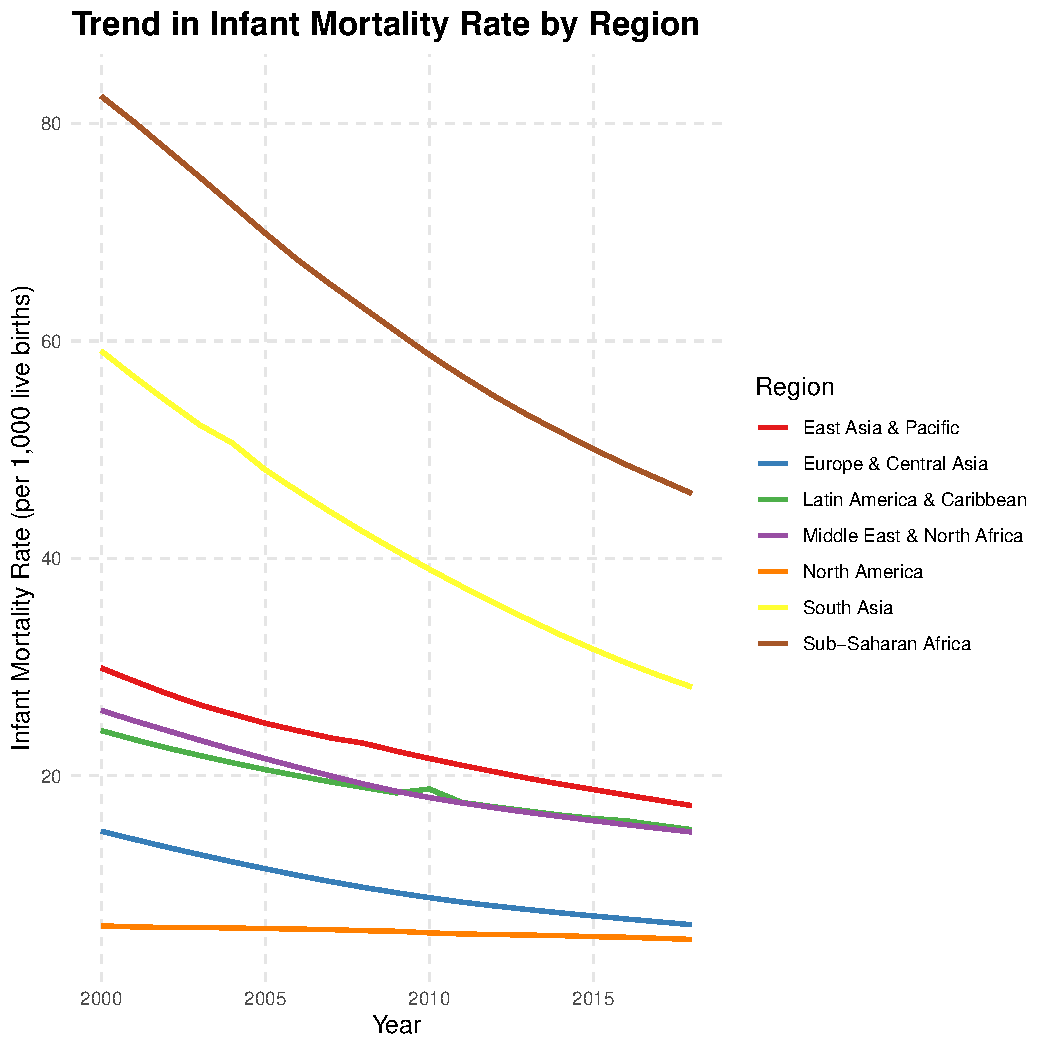
\includegraphics[width=\maxwidth]{figure/unnamed-chunk-9-1} 
\end{knitrout}
\caption{Infant Mortality Rate by Region}
\label{fig}
\end{figure}
The graph displays a overall downward trend in infant mortality rates across different regions of the world from 2000 to 2018.
\begin{itemize}
\item{Sub-Saharan Africa: This region consistently has the highest infant mortality rate, starting around 80 deaths per 1,000 live births in 2000 and gradually declining to around 40 deaths per 1,000 live births in 2018.}

\item{South Asia: This region starts with a slightly lower rate than Sub-Saharan Africa but also experiences a significant decline, ending at approximately 30 deaths per 1,000 live births in 2018.}

\item{East Asia and Pacific: This region demonstrates a substantial decline in infant mortality rate, starting around 60 deaths per 1,000 live births in 2000 and ending around 15 deaths per 1,000 live births in 2018.}

\item{Latin America and Caribbean: This region shows a noticeable decrease in infant mortality rate, starting at around 25 deaths per 1,000 live births in 2000 and ending at about 15 deaths per 1,000 live births in 2018.}

\item{Middle East and North Africa: This region starts with a relatively low infant mortality rate compared to other regions, around 25 deaths per 1,000 live births in 2000, and gradually declines to about 15 deaths per 1,000 live births in 2018.}

\item{Europe and Central Asia: Similar to Middle East and North Africa, this region starts with a low rate and experiences a less steep decline, ending at approximately 10 deaths per 1,000 live births in 2018.}

\item{North America: This region has the lowest infant mortality rate throughout the period, starting at around 7 deaths per 1,000 live births in 2000 and decreasing to about 5 deaths per 1,000 live births in 2018.}
\end{itemize}

\textbf{Overall Observations}
Although notable differences still exist, during the duration of the research project, infant mortality has significantly decreased in every region. South Asia and Sub-Saharan Africa, however, still face significant challenges in this area.

\subsubsection{Birth Rates Year Wise by Region and Income Group}
\begin{lstlisting}
ggplot(world_bank_data, aes(x = Year, y = Birth_Rate, fill = Region)) +
  geom_violin(trim = FALSE, alpha = 0.8) +  
  facet_wrap(~ Income_Group, scales = "free_y") +  
  labs(title = "Birth Rates Year-wise by Region and Income Group",
       x = "Year",
       y = "Birth Rate") +
  theme(
    axis.text.x = element_text(angle = 45, hjust = 1),
    panel.background = element_rect(fill = "white"),
    panel.grid.major = element_line(color = "gray", linetype = "dashed"),
    panel.grid.minor = element_line(color = "gray", linetype = "dotted"),
    plot.title = element_text(hjust = 0.5, size = 16, face = "bold"),
    axis.title = element_text(size = 14),
    legend.position = "bottom",
    legend.title = element_text(size = 12),
    legend.text = element_text(size = 10)
  ) +
  scale_fill_viridis_d(option = "plasma", direction = -1) 



\end{lstlisting}
\newpage
\begin{figure}[h!]
\centering
\begin{knitrout}
\definecolor{shadecolor}{rgb}{0.969, 0.969, 0.969}\color{fgcolor}
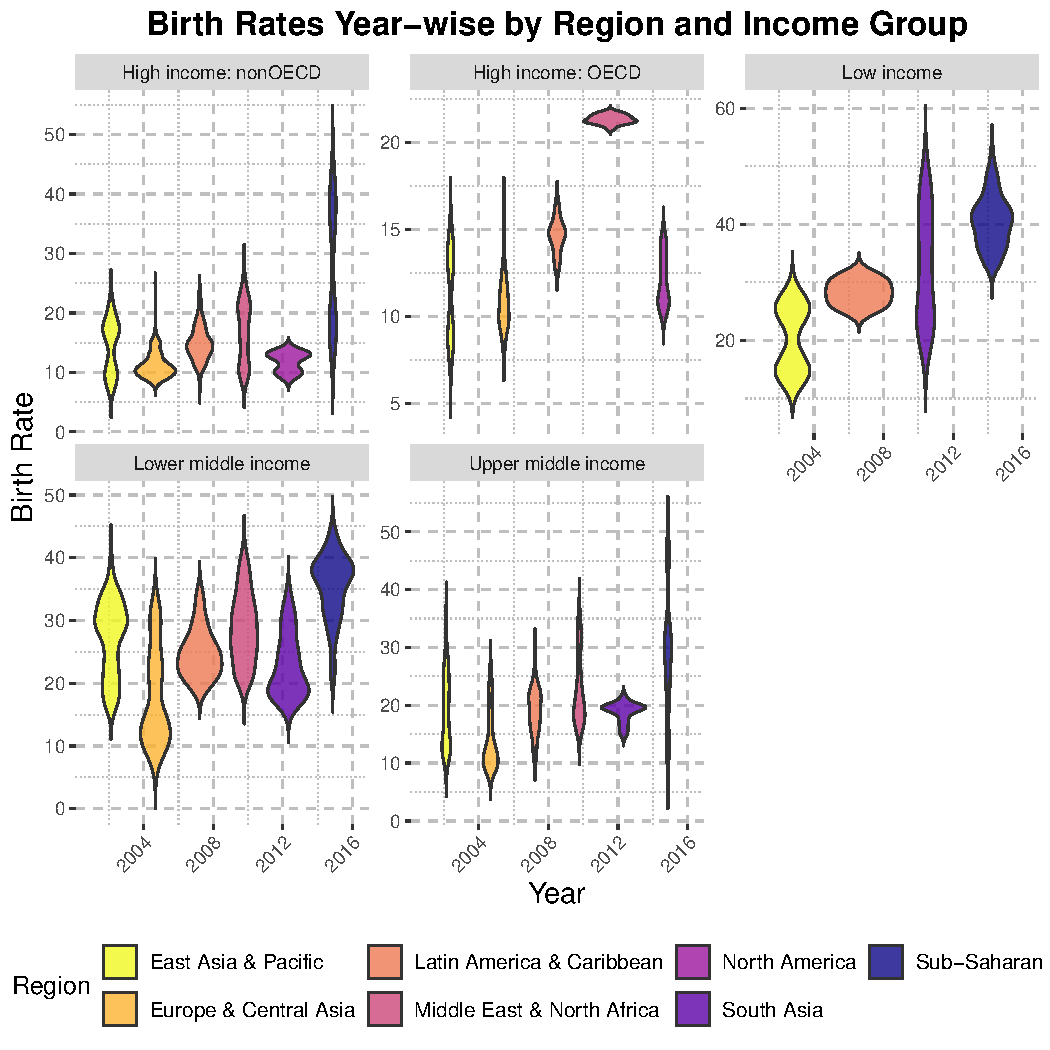
\includegraphics[width=\maxwidth]{figure/unnamed-chunk-10-1} 
\end{knitrout}
\caption{Trend in Birth Rates Year-wise by Region and Income Group}
\label{fig}
\end{figure}
The birth rates of various global areas are displayed in this graphics according to their economic status.\hfill \break

The birth rates for the years 2004, 2008, 2012, and 2016 are plotted according to income level. It demonstrates that during the previous few years, birth rates have steadily declined in the majority of regions. The birth rates do differ throughout the areas, though. For instance, the highest birth rate is found in Sub-Saharan Africa, whereas the lowest is found in North America.\hfill \break

We can also observe some regional trends in birth rate changes:
\begin{itemize}
\item{In high income countries, birth rates seem to be stable with a downward trend.}
\item{In low income countries, birth rates are still decreasing but are still high compared to other regions.}
\item{South Asia is a region that had a high birth rate in 2004 and has seen a significant decrease in birth rates by 2016.}
\item{Lower middle income countries appear to have the most inconsistent trend among income groups.}
\end{itemize}
\textbf{Overall Observation}
Overall, this plot provides insights into the global trends of birth rates across different income levels. It highlights the decline in birth rates in almost all regions, which may be attributed to factors such as economic growth, urbanization, and women's education. It also shows that there are significant regional variations in birth rate trends.

\subsubsection{Death Rates Year Wise by Region and Income Group}
\begin{lstlisting}
ggplot(world_bank_data, aes(x = Year, y = Death_Rate, fill = Region)) +
  geom_violin(trim = FALSE, alpha = 0.8) +  
  facet_wrap(~ Income_Group, scales = "free_y") +  
  labs(title = "Death Rates Year-wise by Region and Income Group",
       x = "Year",
       y = "Death Rate") +
  theme(
    axis.text.x = element_text(angle = 45, hjust = 1),
    panel.background = element_rect(fill = "white"),
    panel.grid.major = element_line(color = "gray", linetype = "dashed"),
    panel.grid.minor = element_line(color = "gray", linetype = "dotted"),
    plot.title = element_text(hjust = 0.5, size = 16, face = "bold"),
    axis.title = element_text(size = 14),
    legend.position = "bottom",
    legend.title = element_text(size = 12),
    legend.text = element_text(size = 10)
  ) +
  scale_fill_viridis_d(option = "Paired", direction = -1) 


\end{lstlisting}
\newpage
\begin{figure}[h!]
\centering
\begin{knitrout}
\definecolor{shadecolor}{rgb}{0.969, 0.969, 0.969}\color{fgcolor}
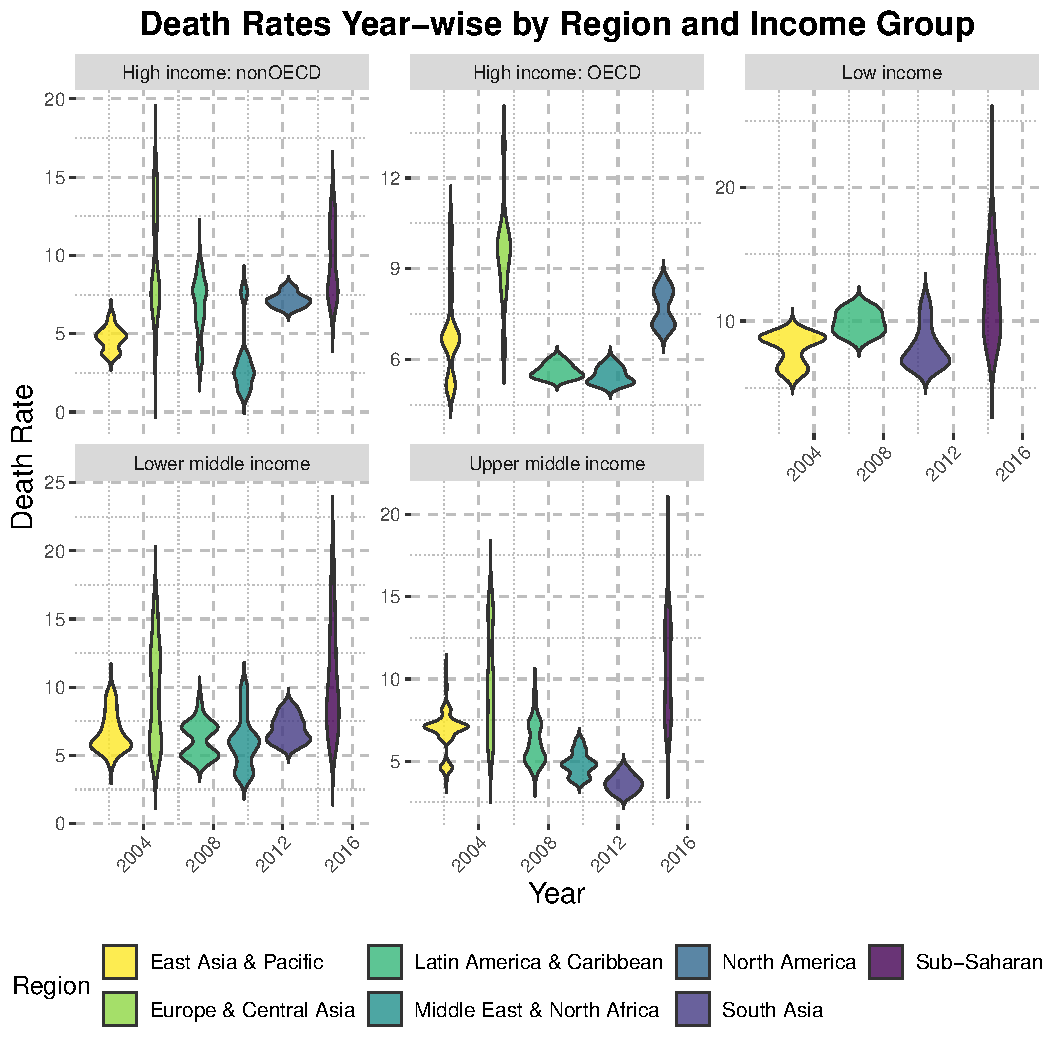
\includegraphics[width=\maxwidth]{figure/unnamed-chunk-11-1} 
\end{knitrout}
\caption{Trend in Death Rates Year-wise by Region and Income Group}
\label{fig}
\end{figure}
The Death rates of various global areas are displayed in this graphics according to their economic status.\hfill \break

The death rates for the years 2004, 2008, 2012, and 2016 are plotted according to income level. It demonstrates that during the previous few years, death rates have steadily declined in the majority of regions. \hfill \break

We can also observe some regional trends in death rate changes:
\begin{itemize}
\item{The death rates in low income countries have stayed relatively stable or even increased in some years.}
\item{Sub-Saharan Africa has a significantly higher death rate compared to other regions with relatively consistent rates.}

\end{itemize}
\textbf{Overall Observation}

This plot provides insights into global trends of death rates across different income levels. It highlights the decline in death rates in most regions, which may be attributed to improvements in healthcare, sanitation, and nutrition. However, the plot also shows that there are significant regional variations in death rate trends. These differences may be due to factors such as economic development, access to healthcare, and disease burden.

\subsubsection{Electric power consumption per capita compare across income groups}
\begin{lstlisting}
electric_gdp_data <- world_bank_data %>%
  select(Electric_Power_Consumption_per_Capita, GDP_per_Capita, Income_Group) %>%
  na.omit()

 ggplot(electric_gdp_data, aes(x = Income_Group, y = Electric_Power_Consumption_per_Capita, fill = Income_Group)) +
  geom_boxplot() +
  scale_y_log10() + 
  labs(title = "Box Plot: Electric Power Consumption by Income Group",
       x = "Income Group",
       y = "Electric Power Consumption (kWh per capita)",
       fill = "Income Group") +
  theme_minimal()


\end{lstlisting}
\newpage
\begin{figure}[h!]
\centering
\begin{knitrout}
\definecolor{shadecolor}{rgb}{0.969, 0.969, 0.969}\color{fgcolor}
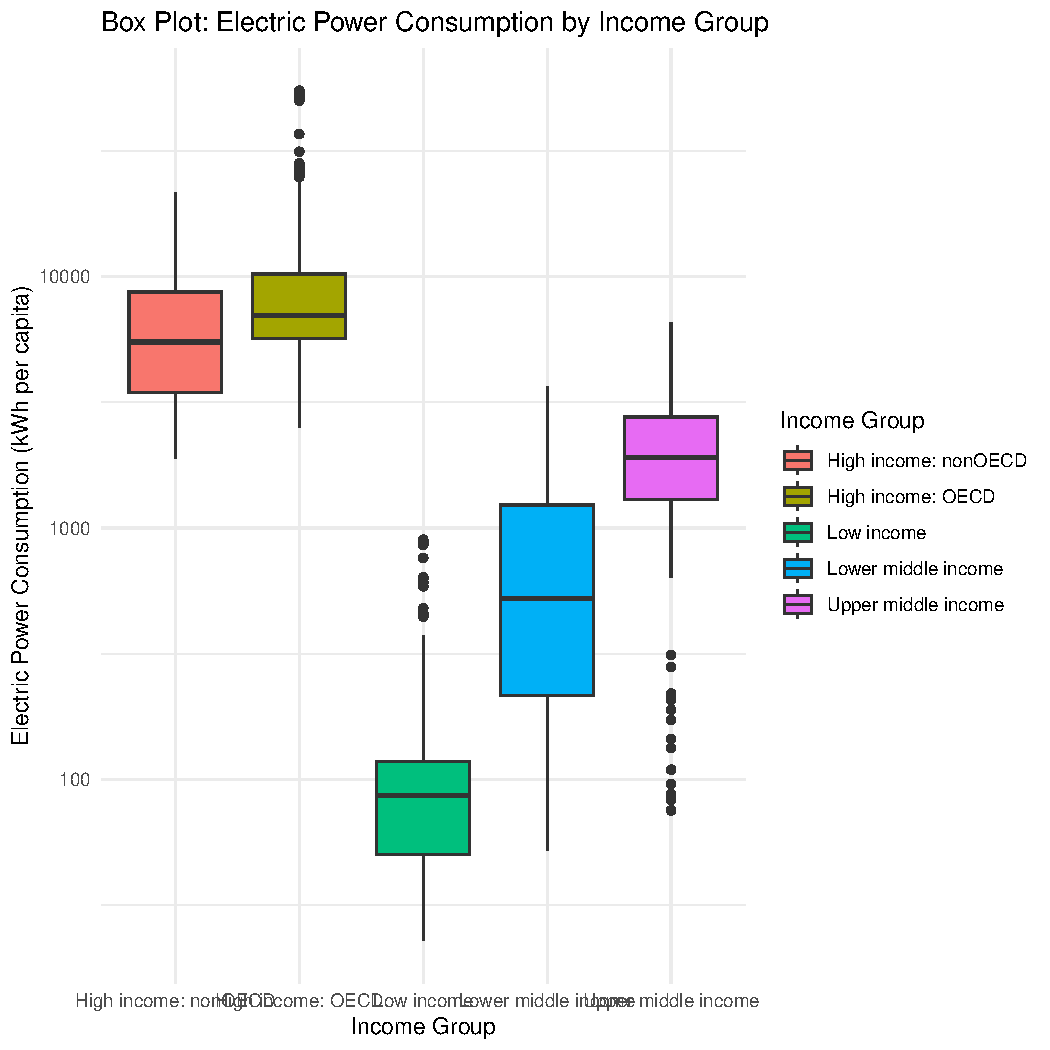
\includegraphics[width=\maxwidth]{figure/unnamed-chunk-12-1} 
\end{knitrout}
\caption{Trend in Electric Power Consumption per Capita by Income Group}
\label{fig}
\end{figure}
The box plot shows the distribution of electric power consumption per capita by income group. 

\textbf{General Trends}
\begin{itemize}
\item{We can see that the median electricity consumption in high-income OECD countries is much higher than that of high-income non-OECD countries. The consumption in high-income OECD countries is also more variable, as indicated by the larger interquartile range.}

\item{The outliers in the plot show that there are some countries in each income group that consume much more or less electricity per capita than the majority of other countries in that group.}
\end{itemize}
\newpage
\subsubsection{Birth Rate and Infant Mortality Rate across Region}
\begin{lstlisting}
ggplot(world_bank_data, aes(x = Birth_Rate, y = Infant_Mortality_Rate)) +
  geom_point(aes(color = Region), alpha = 0.7, size = 3) +
  scale_color_viridis(discrete = TRUE, option = "D", direction = -1) +  
  labs(
    title = "Birth Rate vs. Infant Mortality Rate",
    x = "Birth Rate (per 1000 people)",
    y = "Infant Mortality Rate (per 1000 live births)",
    color = "Region"
  ) +
  theme_minimal() +
  theme(
    plot.title = element_text(size = 18, face = "bold", hjust = 0.5),
    axis.title = element_text(size = 14),
    axis.text = element_text(size = 12),
    legend.position = "bottom",
    legend.title = element_text(size = 14),
    legend.text = element_text(size = 12),
    panel.grid.major = element_line(color = "gray", linetype = "dashed", size = 0.5),
    panel.grid.minor = element_line(color = "gray", linetype = "dashed", size = 0.25)
  )



\end{lstlisting}
\newpage
\begin{figure}[h!]
\centering
\begin{knitrout}
\definecolor{shadecolor}{rgb}{0.969, 0.969, 0.969}\color{fgcolor}
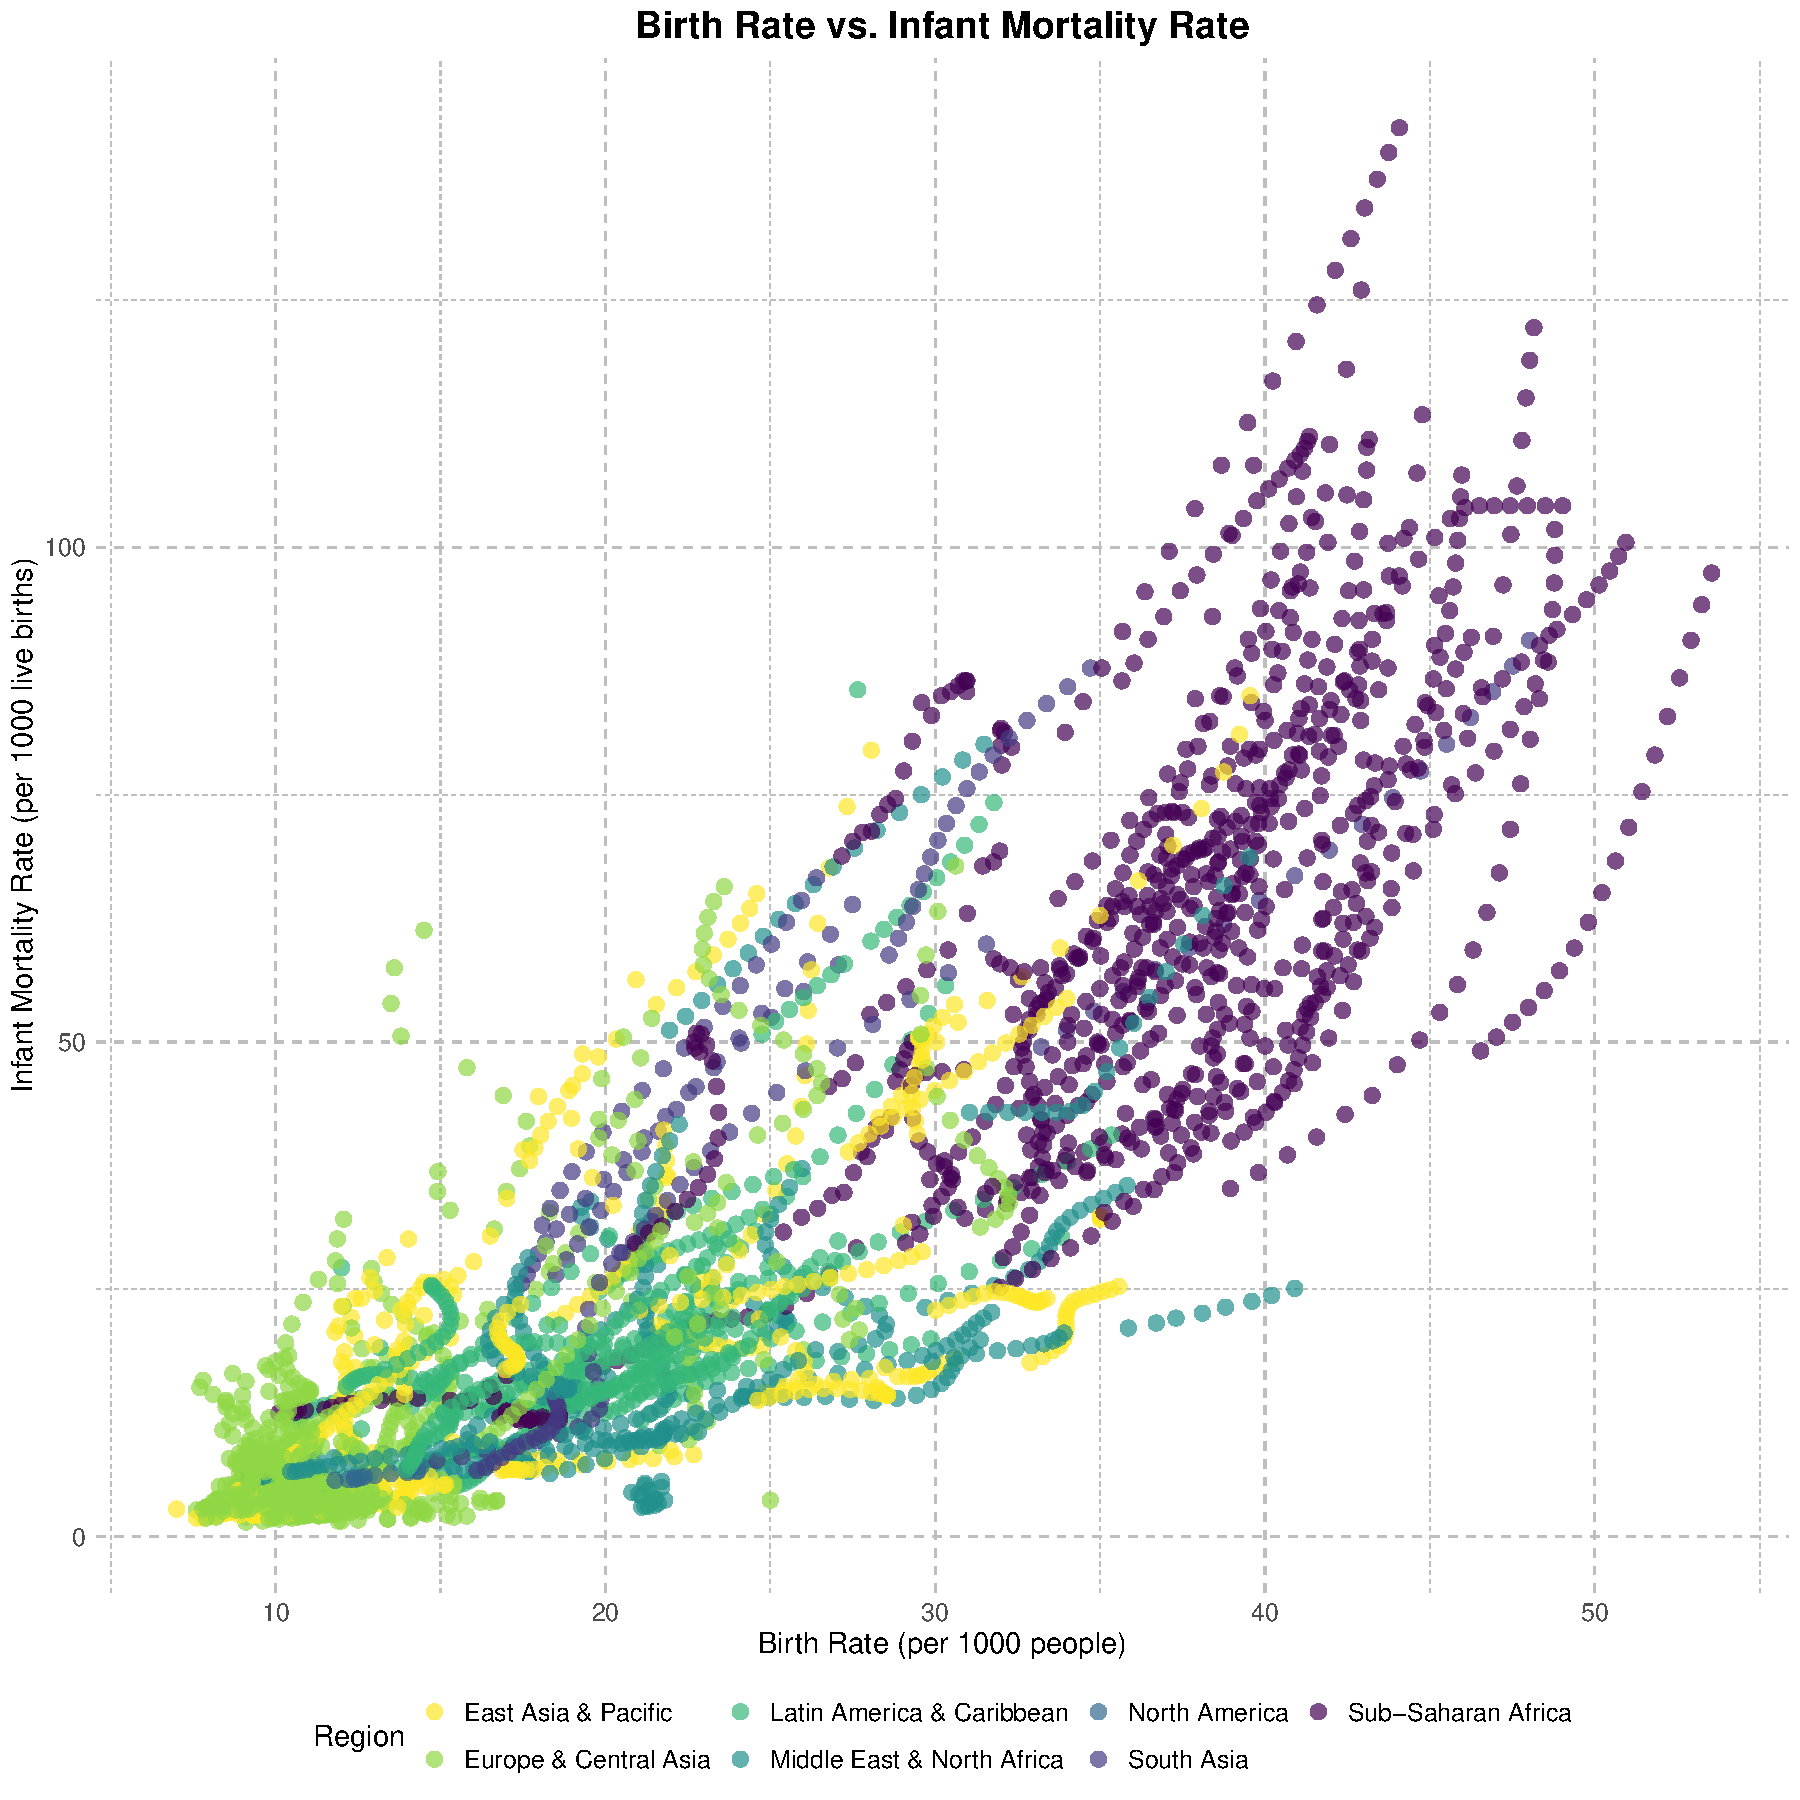
\includegraphics[width=\maxwidth]{figure/unnamed-chunk-13-1} 
\end{knitrout}
\caption{Birth Rate and Infant Mortality Rate across Region}
\label{fig}
\end{figure}
There's a clear positive correlation between birth rate and infant mortality rate. This means that countries with higher birth rates tend to have higher infant mortality rates.
\textbf{Regional Differences}
While the general trend holds true, there are noticeable variations between regions
\begin{itemize}
\item{Sub-Saharan Africa: Has the highest concentration of countries with both high birth rates and high infant mortality rates.}
\item{South Asia: Follows a similar pattern as Sub-Saharan Africa, but with slightly lower infant mortality rates for comparable birth rates.}
\item{East Asia and Pacific, Europe and Central Asia, Latin America and Caribbean: These regions generally exhibit lower birth rates and infant mortality rates compared to the previous two.}
\item{Middle East and North Africa: Shows a more dispersed pattern, with some countries having relatively high infant mortality rates even at lower birth rates.}
\item{North America: Has very few data points, likely due to limited data availability for this region in the dataset.}
\end{itemize}

\subsection{Correlation and Relationships}
\subsubsection{Relationship between internet usage and GDP per capita}
\begin{lstlisting}
correlation <- cor(world_bank_data$Internet_Users_Percentage, world_bank_data$GDP_per_Capita, use="complete.obs")
correlation
ggplot(world_bank_data, aes(x = Internet_Users_Percentage, y = GDP_per_Capita)) +
  geom_point(color = "#336699", size = 2, alpha = 0.7) +  
  geom_smooth(method = "lm", se = FALSE, color = "#FF6600", linetype = "dashed") +  
  labs(
    title = "Relationship between Internet Usage and GDP per Capita",
    subtitle = paste0("Correlation: ", round(correlation, 3)),  
    x = "Internet Users Percentage",
    y = "GDP per Capita (USD)"  
  ) +
  theme_bw() +  
  theme(
    plot.title = element_text(size = 18, face = "bold"),
    plot.subtitle = element_text(size = 14),
    axis.title = element_text(size = 14),
    axis.text = element_text(size = 12),
    panel.grid.major = element_line(color = "#EEEEEE"),
    panel.grid.minor = element_line(color = "#EEEEEE")
  )

\end{lstlisting}
\newpage
\begin{figure}[h!]
\centering
\begin{knitrout}
\definecolor{shadecolor}{rgb}{0.969, 0.969, 0.969}\color{fgcolor}\begin{kframe}
\begin{verbatim}
## [1] 0.6794173
\end{verbatim}
\end{kframe}
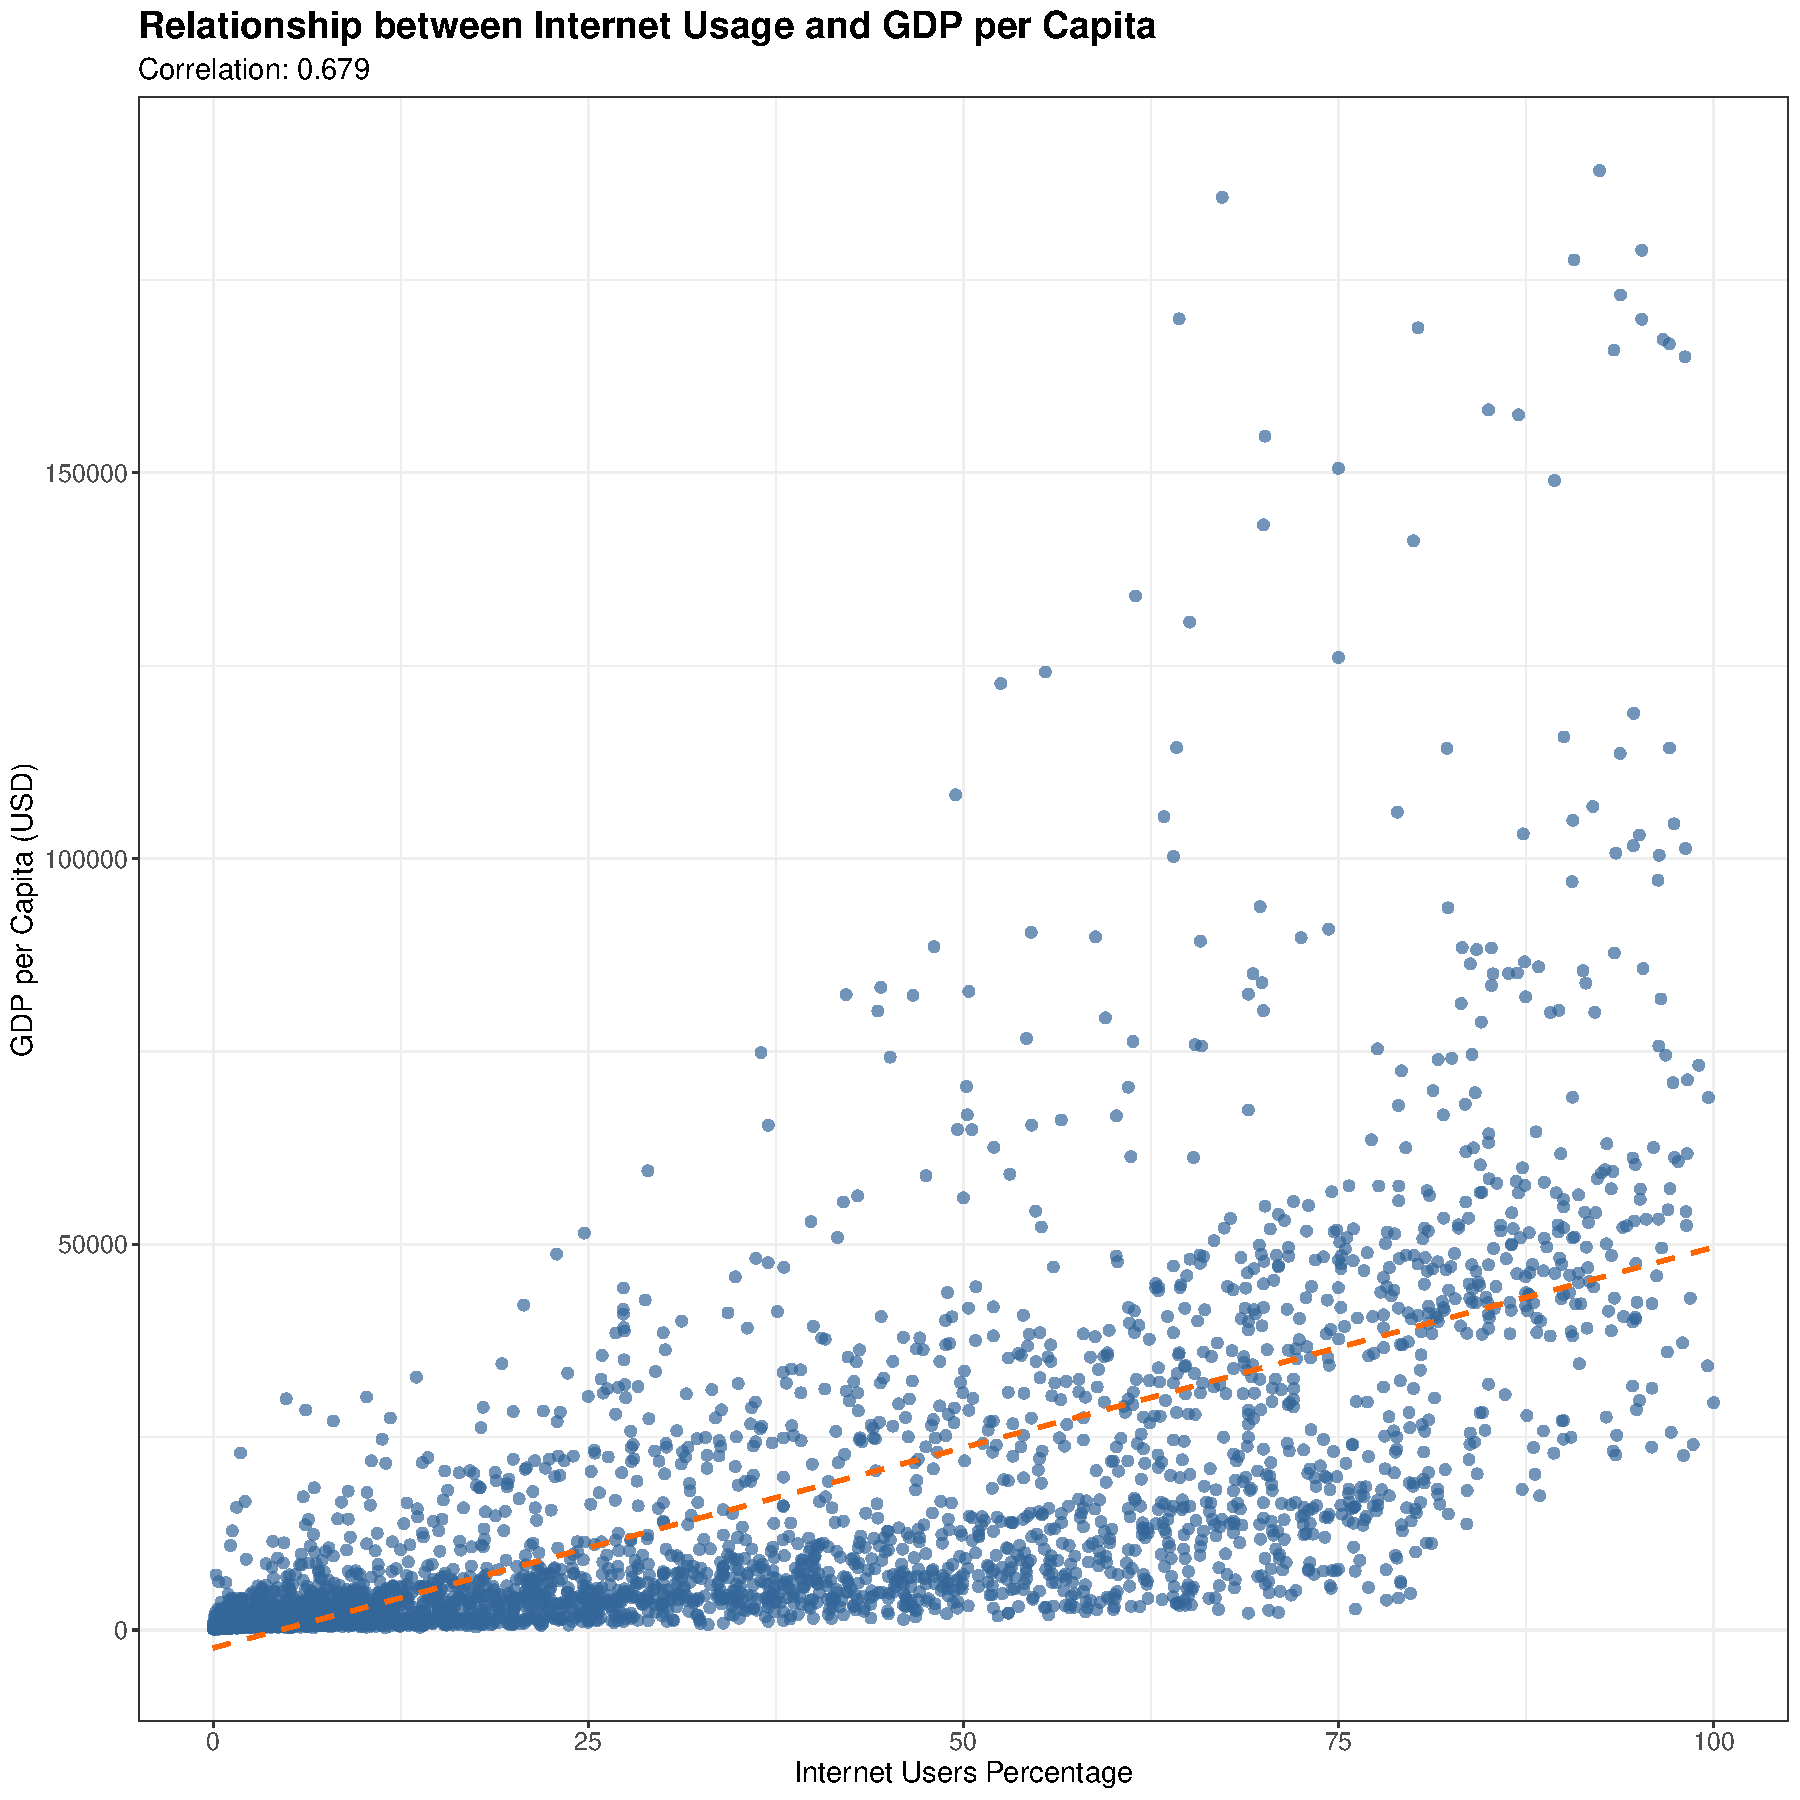
\includegraphics[width=\maxwidth]{figure/unnamed-chunk-14-1} 
\end{knitrout}
\caption{Relationship between internet usage and GDP per capita}
\label{fig}
\end{figure}
The plot visualizes the relationship between Internet Usage (as a percentage of the population) and GDP per capita (in USD) across different countries. Here's a breakdown of the insights: 


\textbf{Positive Correlation}

\begin{itemize}
\item{The upward trend of the data points and the orange line indicate a positive correlation between internet usage and GDP per capita. This means that as internet usage increases in a country, its GDP per capita tends to increase as well.}
\end{itemize}

\textbf{Strength of Correlation}

\begin{itemize}
\item{The correlation coefficient of 0.679 suggests a moderately strong positive relationship. While not perfectly linear, the relationship is noticeable. }
\end{itemize}

\textbf{Outliers}
\begin{itemize}
\item{There are some outliers in the data.  For instance, some countries with relatively high internet usage have lower GDP per capita, and vice versa.}
\end{itemize}

\textbf{Overall Observation}

The plot suggests a link between internet usage and GDP per capita, but further investigation is needed to understand the underlying reasons for this relationship. 

\subsubsection{Correlations among various socio-economic variables}
\begin{lstlisting}
cor_matrix <- cor(world_bank_data[, c("Birth_Rate", "Death_Rate", 
                                      "Electric_Power_Consumption_per_Capita", "GDP_per_Capita", 
                                      "Internet_Users_Percentage", "Infant_Mortality_Rate", 
                                      "Life_Expectancy", "Population_Density", 
                                      "Unemployment_Rate")
], use = "pairwise.complete.obs")


cor_data <- melt(cor_matrix)


ggplot(data = cor_data, aes(x = Var1, y = Var2, fill = value)) +
  geom_tile(color = "white", size = 0.5) + 
  scale_fill_viridis(option = "magma", name = "Correlation") + 
  geom_text(aes(label = round(value, 2)), color = "white", size = 4) +
  labs(x = "", y = "") +
  ggtitle("Correlation Heatmap of World Bank Data") +
  theme_minimal() +  
  theme(
    axis.text.x = element_text(angle = 45, hjust = 1, size = 10, vjust = 1, face = "bold"),
    axis.text.y = element_text(size = 10, face = "bold"),
    axis.title = element_blank(),  
    panel.background = element_blank(),
    panel.grid.major = element_line(color = "grey80", size = 0.2),  
    panel.grid.minor = element_blank(),
    plot.title = element_text(hjust = 0.5, size = 16, face = "bold"),
    legend.position = "bottom",
    legend.text = element_text(size = 10, face = "bold"),
    legend.title = element_text(size = 12, face = "bold")
  ) +
  coord_fixed()


\end{lstlisting}
\newpage
\begin{figure}[h!]
\centering
\begin{knitrout}
\definecolor{shadecolor}{rgb}{0.969, 0.969, 0.969}\color{fgcolor}
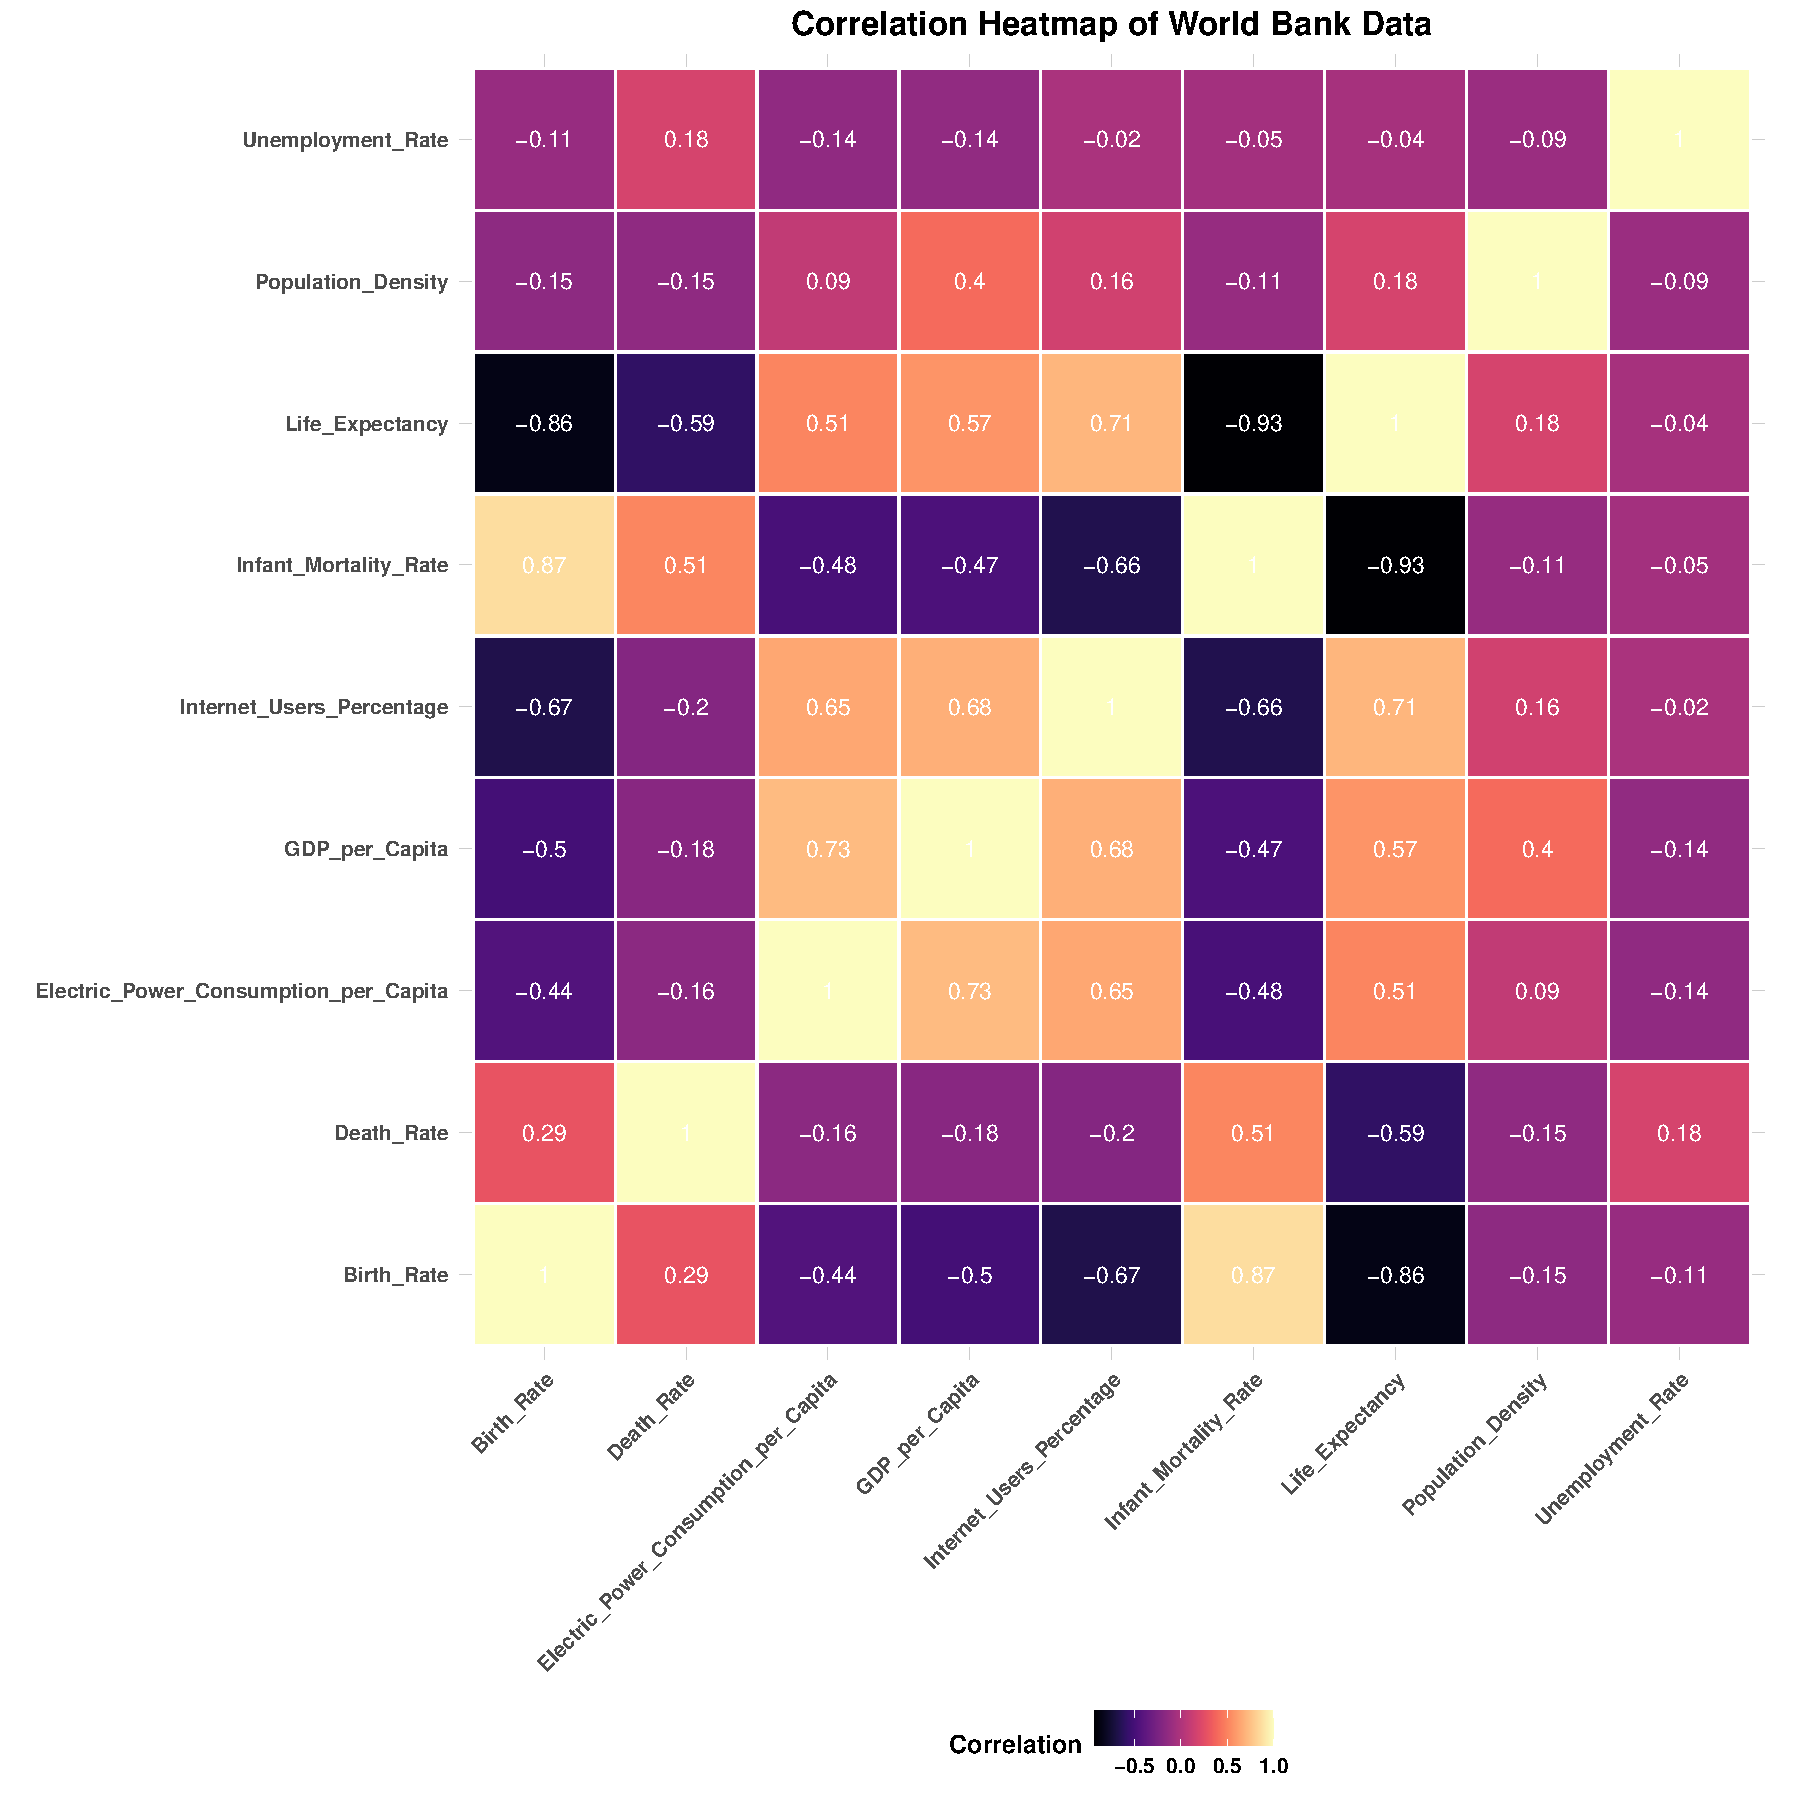
\includegraphics[width=\maxwidth]{figure/unnamed-chunk-15-1} 
\end{knitrout}
\caption{Correlation Heatmap of World Bank Data}
\label{fig}
\end{figure}
This heatmap visualizes the correlation between various global metrics based on World Bank data.The heatmap's squares each reflect the correlation coefficient—the color of which denotes the correlation's strength and direction—between two variables. The insights are broken down into detail here:

\textbf{Insights:}
\begin{itemize}
\item{Life Expectancy vs. Infant Mortality Rate: Strong negative correlation (dark purple).This indicates that as life expectancy increases, the infant mortality rate tends to decrease significantly.}

\item{GDP per Capita vs. Life Expectancy:Strong positive correlation (yellow). Higher GDP per capita is associated with higher life expectancy.}

\item{Internet Users Percentage vs. GDP per Capita: Moderate positive correlation (orange). Countries with higher GDP per capita generally have a higher percentage of internet users.}

\item{Electric Power Consumption per Capita vs. GDP per Capita:Strong positive correlation (yellow). This suggests that higher GDP per capita is linked with higher electric power consumption per capita.}

\item{Birth Rate vs. Infant Mortality Rate:Moderate positive correlation (orange). Higher birth rates are associated with higher infant mortality rates.}

\item{Death Rate vs. Birth Rate:Moderate positive correlation (Red). Countries with higher birth rates also tend to have higher death rates.}

\item{Life Expectancy vs. Birth Rate:Strong negative correlation (dark purple). Higher life expectancy is associated with lower birth rates.}

\item{Unemployment Rate vs. GDP per Capita:Negative correlation (light purple). Higher GDP per capita tends to be associated with lower unemployment rates, though this correlation is not very strong.}

\item{Population Density vs. Internet Users Percentage:Weak positive correlation (red). Higher population density shows a slight tendency towards a higher percentage of internet users.}

\item{Internet Users Percentage vs. Life Expectancy:Moderate positive correlation (orange). Higher internet usage is associated with higher life expectancy.}
\end{itemize}
The heatmap reveals significant relationships between economic, social, and health metrics. Notably, life expectancy, GDP per capita, and internet usage are strongly interconnected. In contrast, high birth rates are linked with high infant mortality and death rates. These insights are crucial for understanding how various factors influence development and quality of life across different countries.

\newpage
\section{Geography Visualization}
\subsection{Average Birth Rate Map}
\begin{lstlisting}
average_birth_rate <- world_bank_data %>%
  group_by(Country) %>%
  summarise(Birth_Rate = mean(Birth_Rate, na.rm = TRUE))


BR <- joinCountryData2Map(average_birth_rate, joinCode = "NAME", nameJoinColumn = "Country")


birth_rate_map <- mapCountryData(BR, nameColumnToPlot = "Birth_Rate", mapTitle = "Average Birth Rate (2000-2018)", 
                                 colourPalette = "heat", missingCountryCol = "black")

\end{lstlisting}
This map visualizes the average birth rate per country from 2000 to 2018. The color scale at the bottom indicates the birth rate, with lighter colors representing lower birth rates and darker colors representing higher birth rates.The country without any data is represented in black.
\newpage

\begin{figure}[h!]
\centering
\begin{knitrout}
\definecolor{shadecolor}{rgb}{0.969, 0.969, 0.969}\color{fgcolor}\begin{kframe}
\begin{verbatim}
## 204 codes from your data successfully matched countries in the map
## 7 codes from your data failed to match with a country code in the map
## 39 codes from the map weren't represented in your data
\end{verbatim}
\end{kframe}
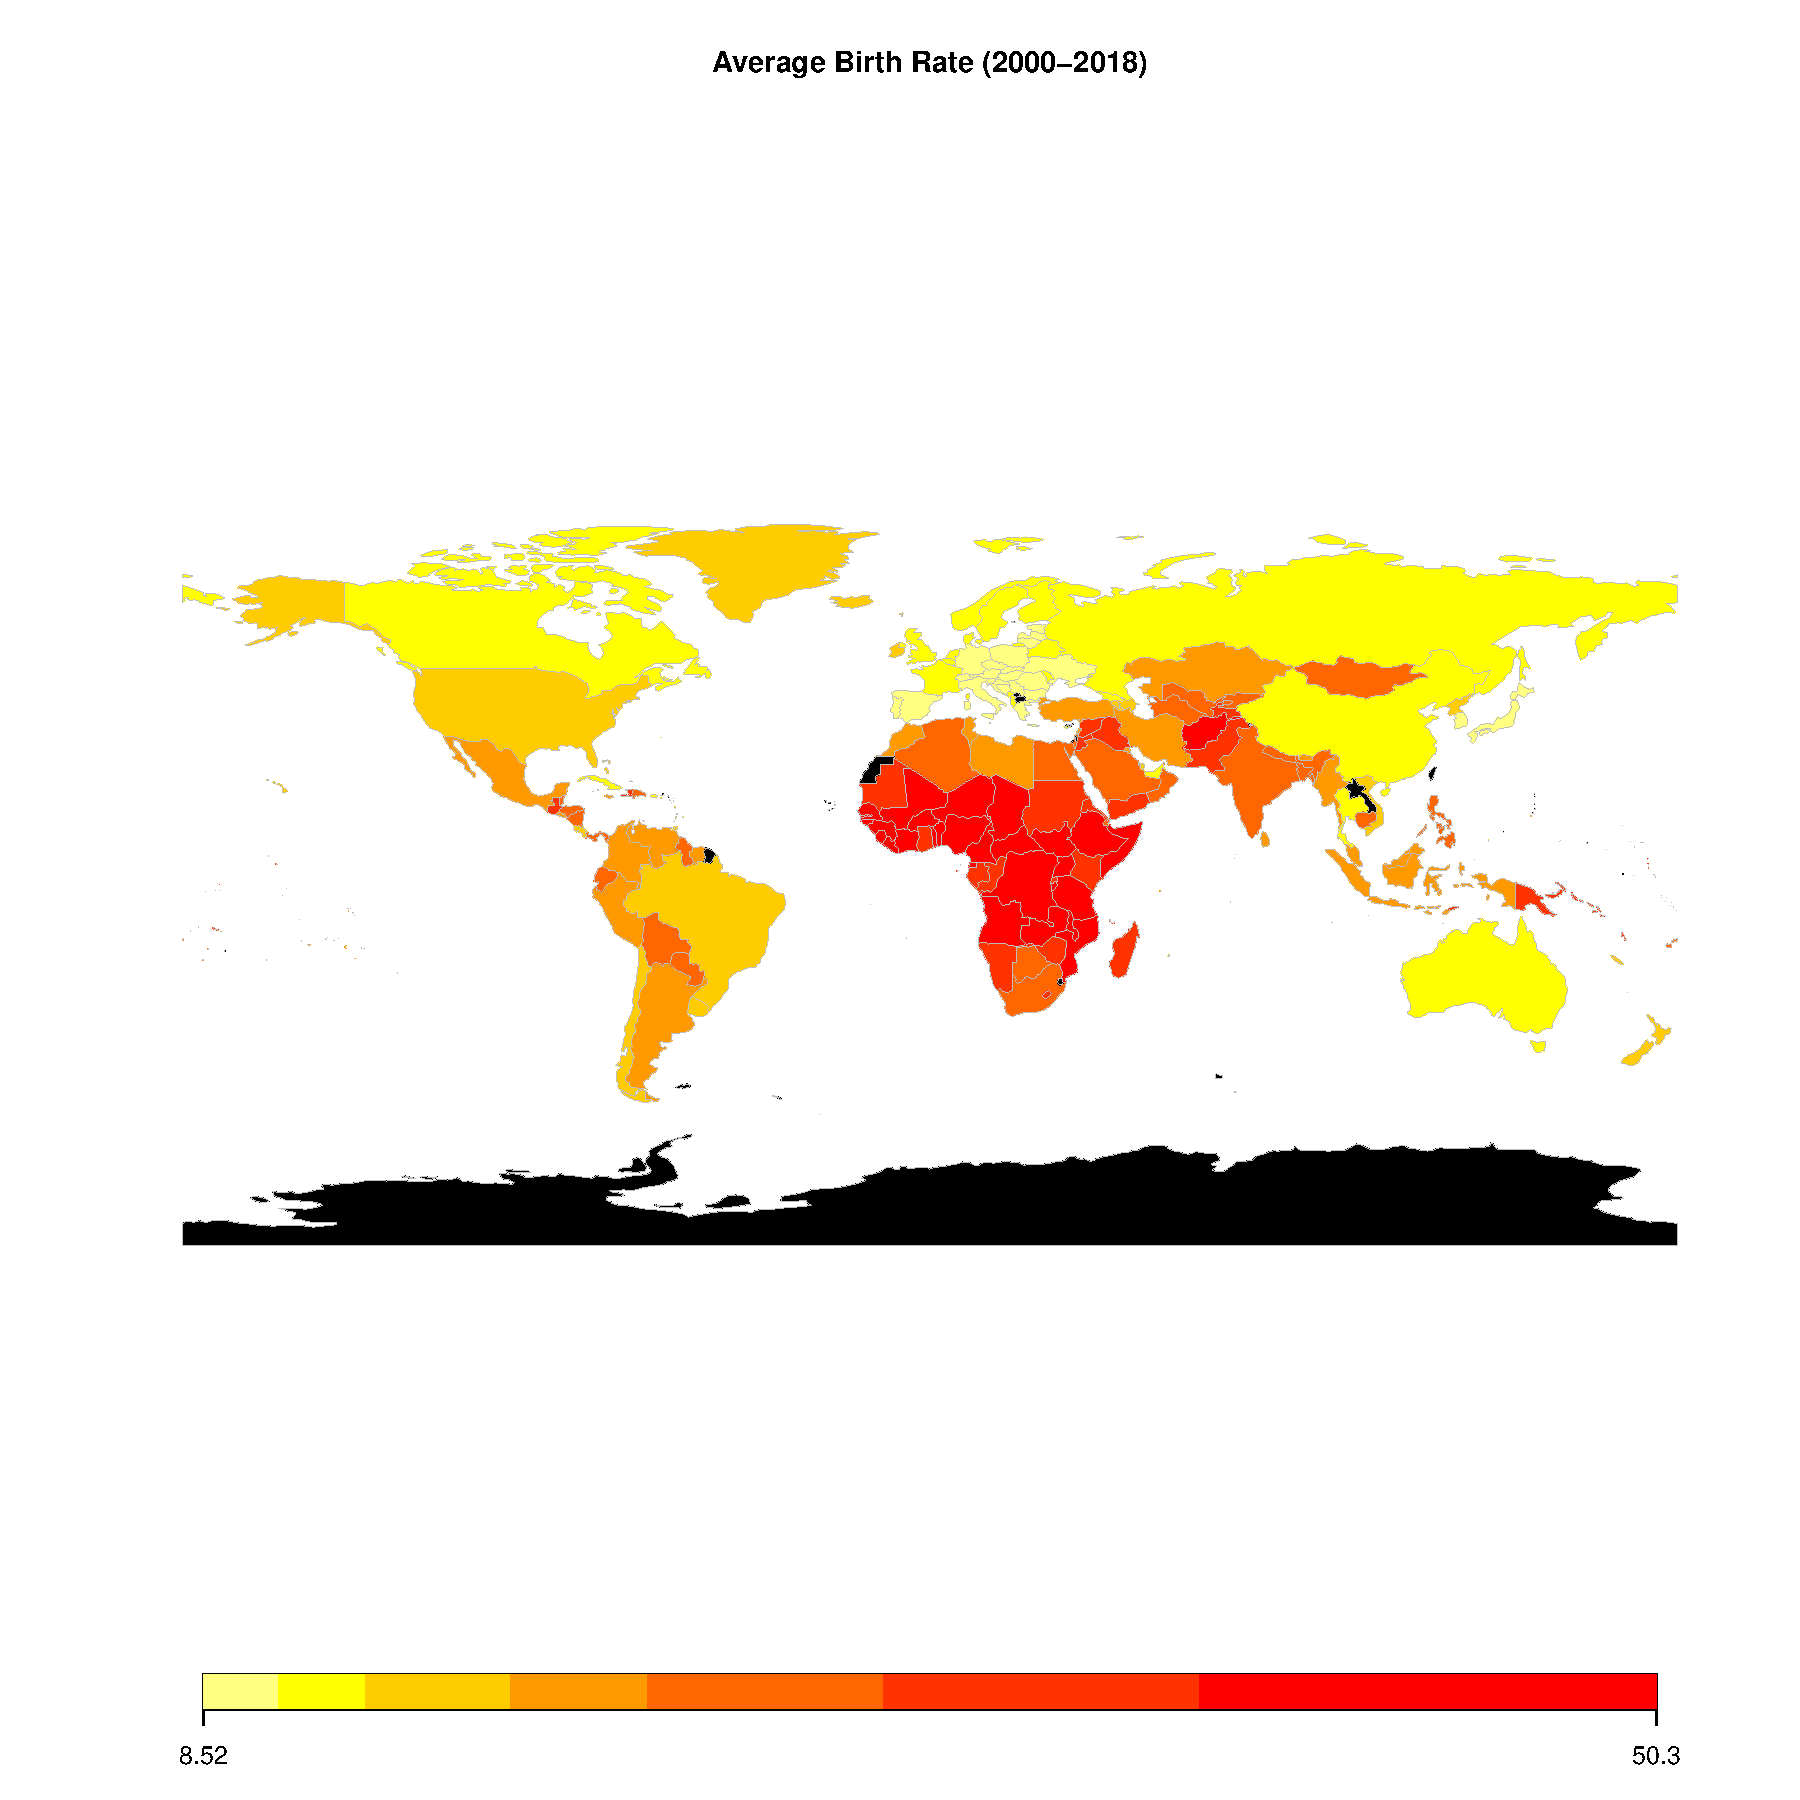
\includegraphics[width=\maxwidth]{figure/unnamed-chunk-16-1} 
\end{knitrout}
\caption{Map Representing Average Birth Rate}

\label{fig}
\end{figure}


\newpage
\subsection{Average Death Rate Map}
\begin{lstlisting}
average_death_rate <- world_bank_data %>%
  group_by(Country) %>%
  summarise(Death_Rate = mean(Death_Rate, na.rm = TRUE))


DR <- joinCountryData2Map(average_death_rate, joinCode = "NAME", nameJoinColumn = "Country")


death_rate_map <- mapCountryData(DR, nameColumnToPlot = "Death_Rate", mapTitle = "Average Death Rate (2000-2018)", 
                                 colourPalette = "white2Black", missingCountryCol = "white")

\end{lstlisting}
This map visualizes the average death rate per country from 2000 to 2018. The color scale at the bottom indicates the birth rate, with grayish color representing lower birth rates and darker colors representing higher death rates.The country without any data is represented in white.
\newpage
\begin{figure}[h!]

\centering
\begin{knitrout}
\definecolor{shadecolor}{rgb}{0.969, 0.969, 0.969}\color{fgcolor}\begin{kframe}
\begin{verbatim}
## 204 codes from your data successfully matched countries in the map
## 7 codes from your data failed to match with a country code in the map
## 39 codes from the map weren't represented in your data
\end{verbatim}
\end{kframe}
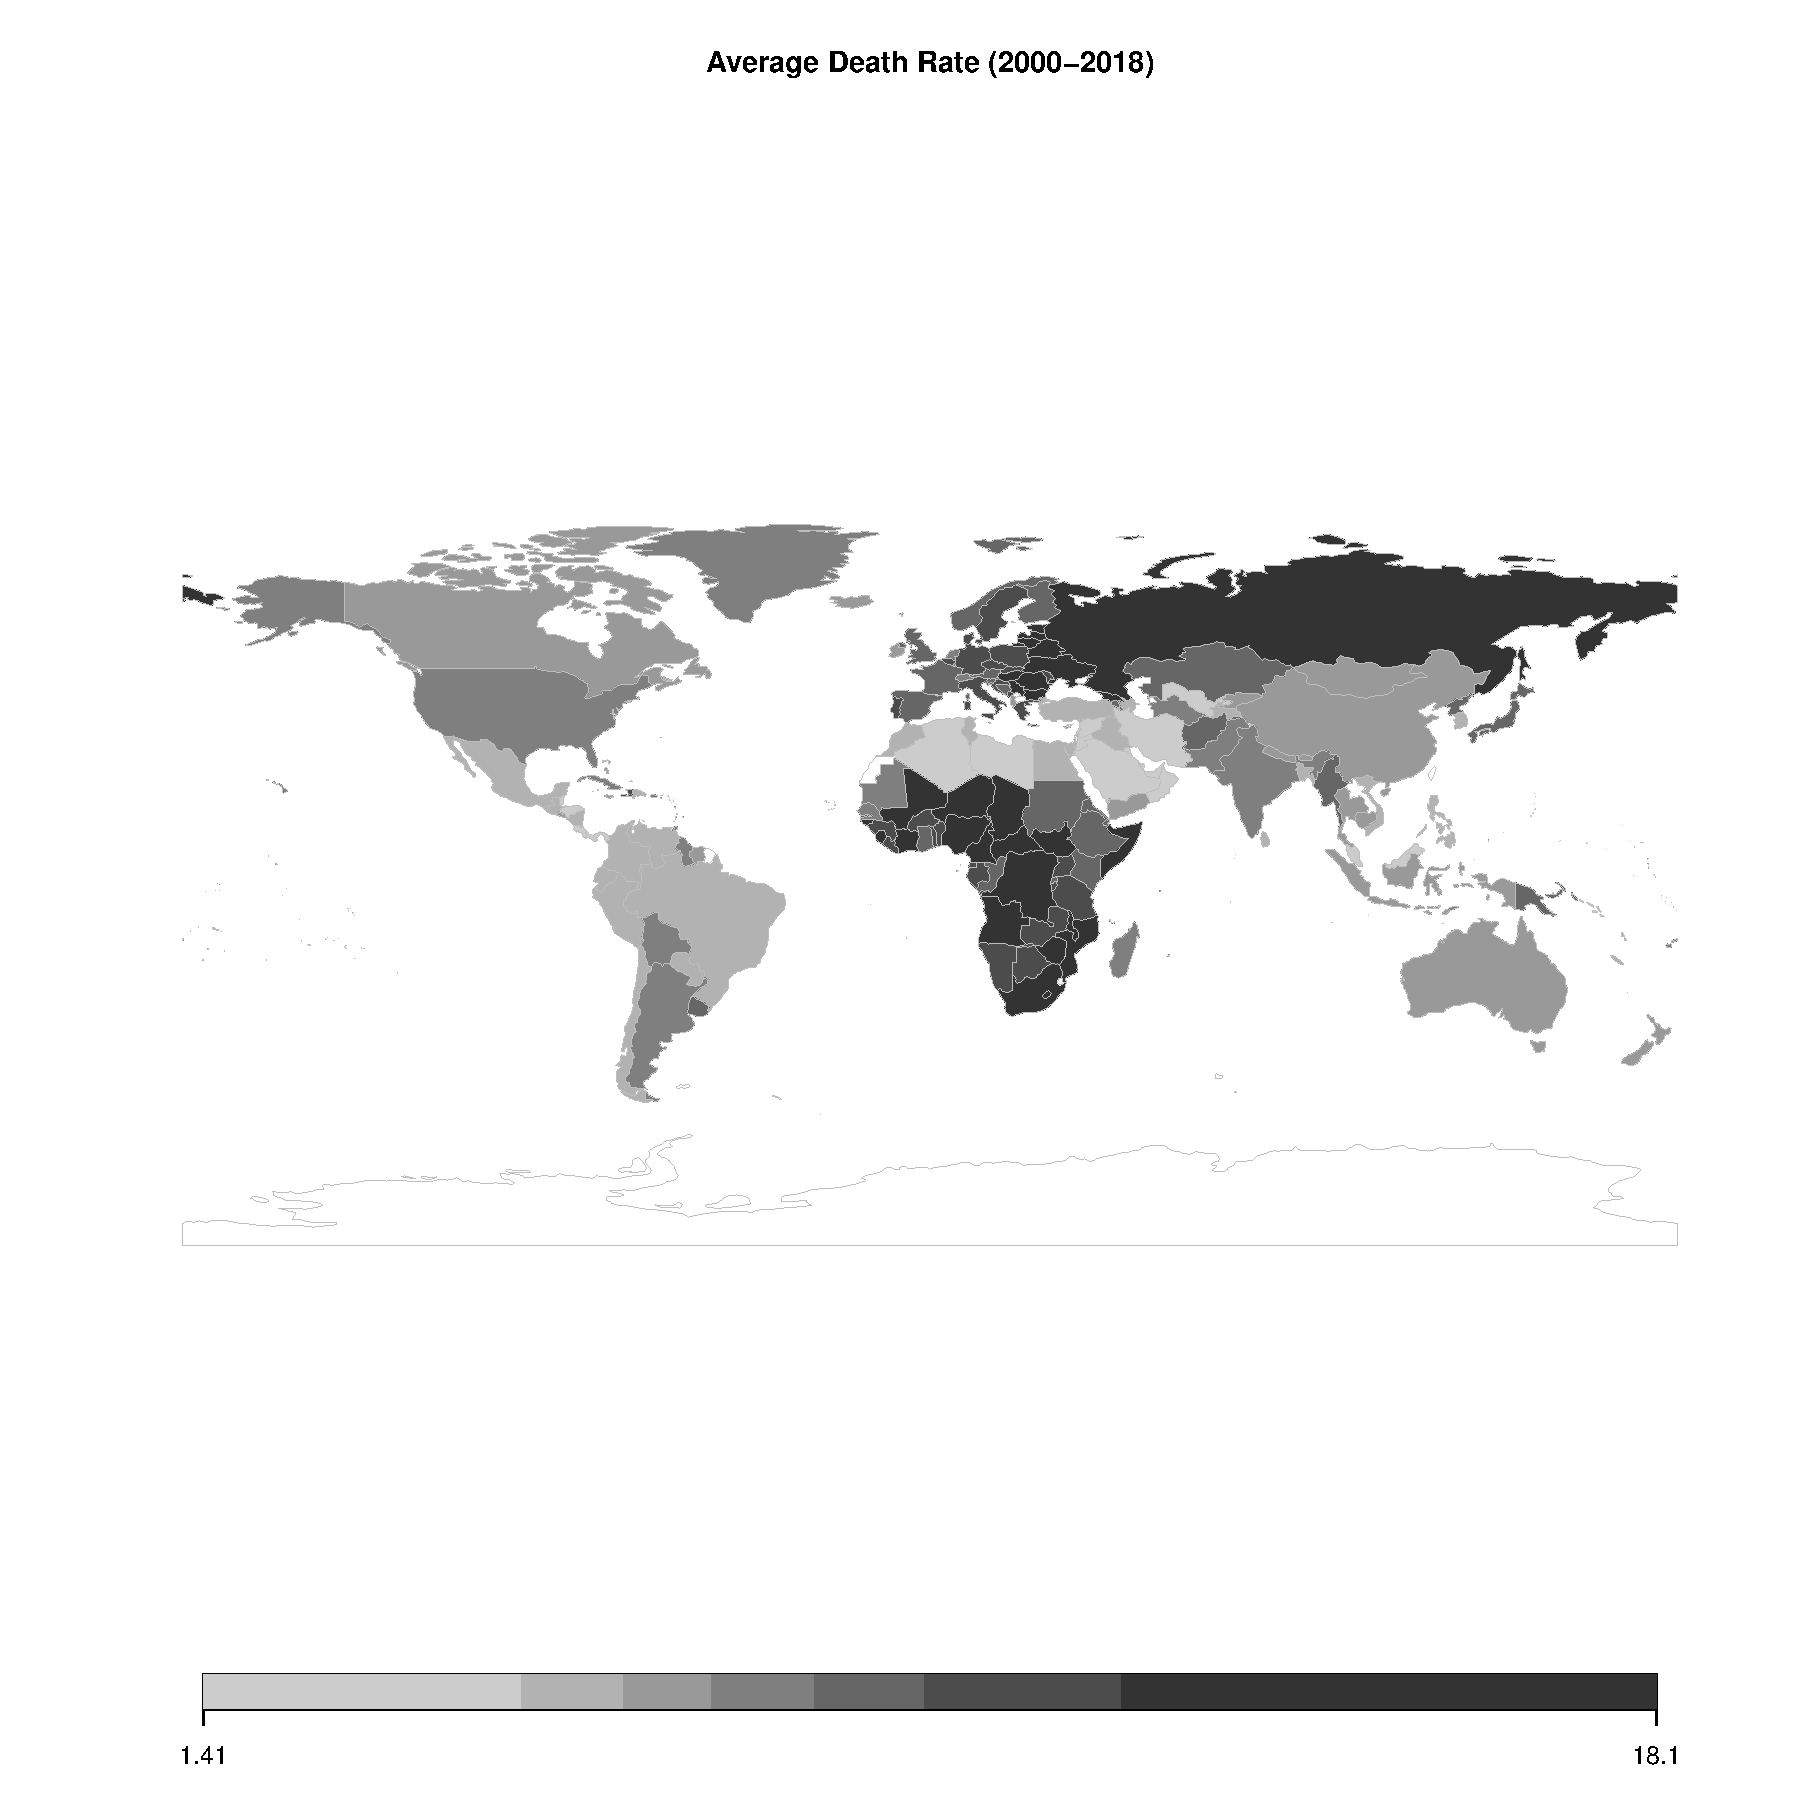
\includegraphics[width=\maxwidth]{figure/unnamed-chunk-17-1} 
\end{knitrout}
\caption{Map Representing Average Death Rate}

\label{fig}
\end{figure}



\newpage
\subsection{Average Electric Power Consumption per Captia Map}
\begin{lstlisting}
average_electric_power<- world_bank_data %>%
  group_by(Country) %>%
  summarise(Electric_Power_Consumption_per_Capita = mean(Electric_Power_Consumption_per_Capita, na.rm = TRUE))

EPR <- joinCountryData2Map(average_electric_power, joinCode = "NAME", nameJoinColumn = "Country")


electric_power_map <- mapCountryData(EPR, nameColumnToPlot = "Electric_Power_Consumption_per_Capita", mapTitle = " Average Electric Power Consumption (kWh per capita 2000-2018)", 
                                     colourPalette = "diverging", missingCountryCol = "black")

\end{lstlisting}
This map shows the average electric power consumption per capita (measured in kilowatt-hours per capita) from 2000 to 2018 for countries around the world. The color scale at the bottom indicates the range of consumption, with:
\begin{itemize}
\item{Dark blue representing the lowest consumption (33.6 kWh per capita).}
\item{Yellow, white and green representing mid-range consumption.}
\item{Red is representing the highest consumption (up to 40,000 kWh per capita).}
\item{The country with no data is represented in black.}
\end{itemize}
Countries with higher electric power consumption per capita are predominantly in North America, Europe, and Oceania, whereas many countries in Africa and parts of Asia have lower consumption.

\newpage
\begin{figure}[h!]
\centering
\begin{knitrout}
\definecolor{shadecolor}{rgb}{0.969, 0.969, 0.969}\color{fgcolor}\begin{kframe}
\begin{verbatim}
## 204 codes from your data successfully matched countries in the map
## 7 codes from your data failed to match with a country code in the map
## 39 codes from the map weren't represented in your data
\end{verbatim}
\end{kframe}
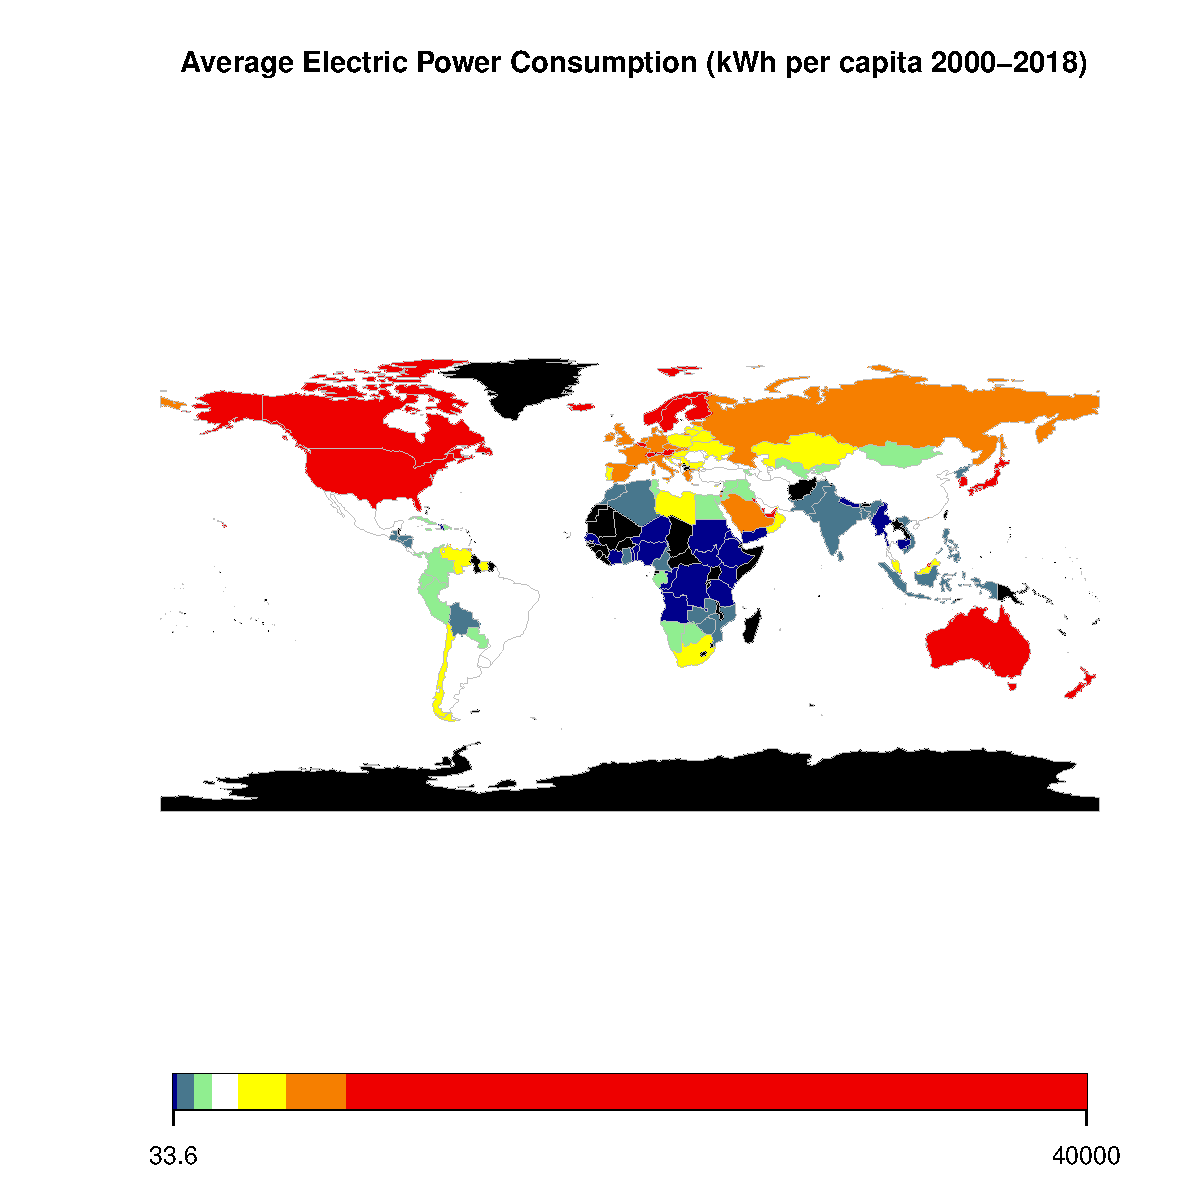
\includegraphics[width=\maxwidth]{figure/unnamed-chunk-18-1} 
\end{knitrout}
\caption{Map Representing Average Electric Power Consumption per Captia }

\label{fig}
\end{figure}

\newpage

\subsection{Average GDP Map}
\begin{lstlisting}
average_GDP<- world_bank_data %>%
  group_by(Country) %>%
  summarise(GDP = mean(GDP, na.rm = TRUE))


GDPM <- joinCountryData2Map(average_GDP, joinCode = "NAME", nameJoinColumn = "Country")


GDP_map <- mapCountryData(GDPM, nameColumnToPlot = "GDP", mapTitle = " Average GDP", 
                                     colourPalette = "topo", missingCountryCol = "black")

\end{lstlisting}
This map visualizes the average GDP per country from 2000 to 2018. The color scale at the bottom indicates the GDP, with skyblue color representing lower birth rates and dark purple color representing higher death rates.The country without any data is represented in black.
\newpage
\begin{figure}[h!]
\centering
\begin{knitrout}
\definecolor{shadecolor}{rgb}{0.969, 0.969, 0.969}\color{fgcolor}\begin{kframe}
\begin{verbatim}
## 204 codes from your data successfully matched countries in the map
## 7 codes from your data failed to match with a country code in the map
## 39 codes from the map weren't represented in your data
\end{verbatim}
\end{kframe}
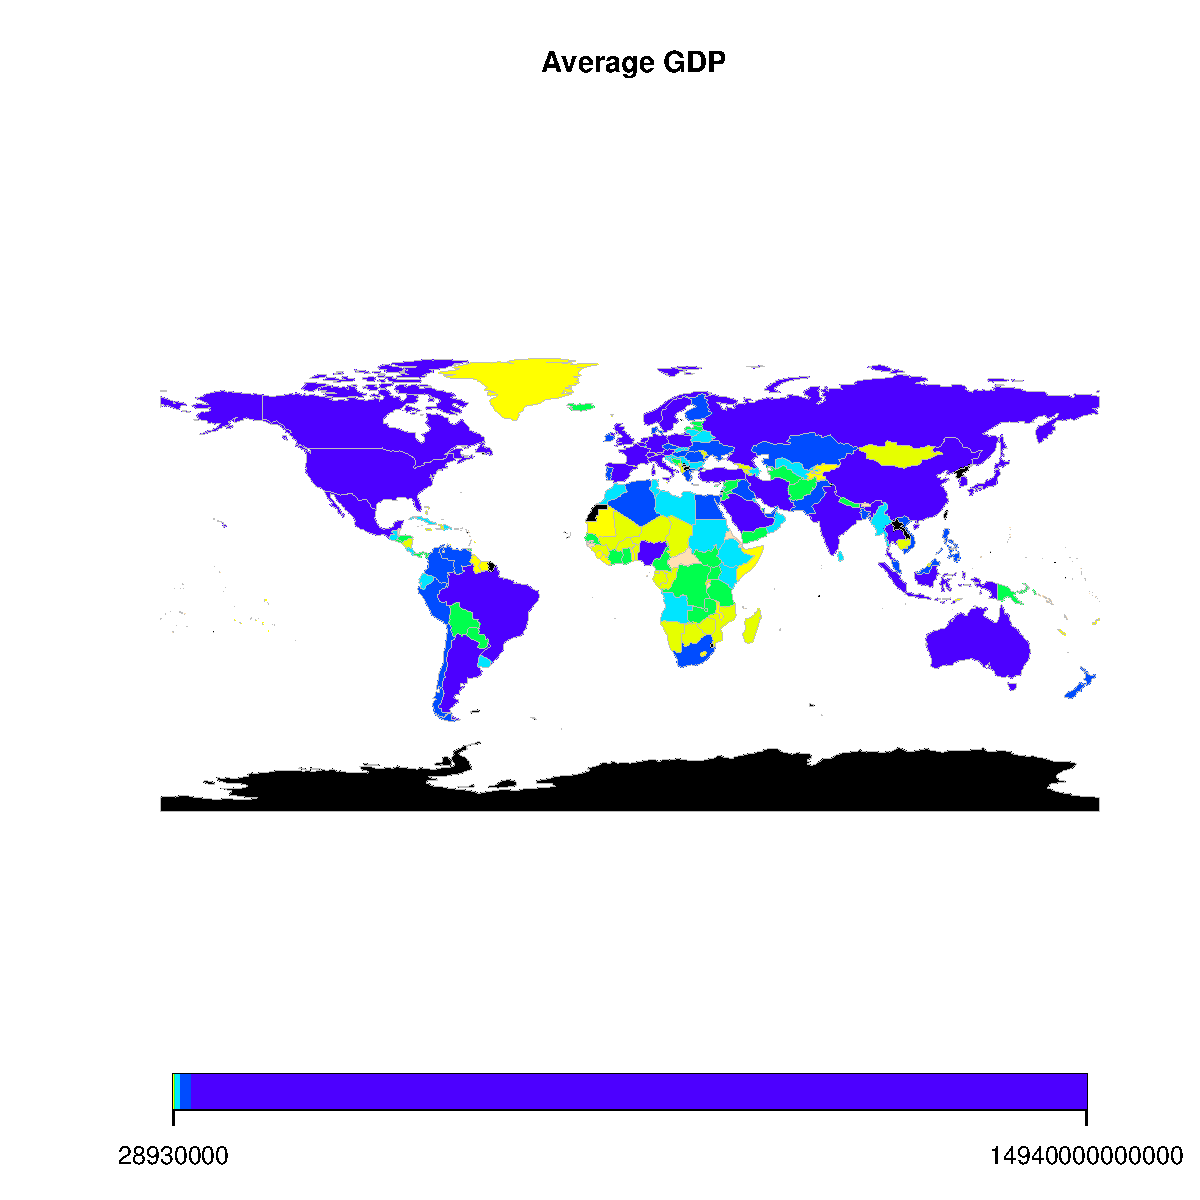
\includegraphics[width=\maxwidth]{figure/unnamed-chunk-19-1} 
\end{knitrout}
\caption{Map Representing Average GDP }

\label{fig}
\end{figure}


\newpage
\subsection{Average GDP per Capita Map}
\begin{lstlisting}
average_gdp_per_capita<- world_bank_data %>%
  group_by(Country) %>%
  summarise(GDP_per_Capita = mean(GDP_per_Capita, na.rm = TRUE))


GDPPC <- joinCountryData2Map(average_gdp_per_capita, joinCode = "NAME", nameJoinColumn = "Country")


GDPC_map <- mapCountryData(GDPPC, nameColumnToPlot = "GDP_per_Capita", mapTitle = "Average GDP Per Capita", 
                                     colourPalette = "rainbow", missingCountryCol = "black")

\end{lstlisting}
This map shows the average GDP per capita of countries around the world. The countries with the highest GDP per capita are in red, and the countries with the lowest GDP per capita are in pink. The map shows that the wealthiest countries are located in North America, Europe, and Australia. The poorest countries are located in Africa and South America.The country without any data is represented in black.
\newpage
\begin{figure}[h!]
\centering
\begin{knitrout}
\definecolor{shadecolor}{rgb}{0.969, 0.969, 0.969}\color{fgcolor}\begin{kframe}
\begin{verbatim}
## 204 codes from your data successfully matched countries in the map
## 7 codes from your data failed to match with a country code in the map
## 39 codes from the map weren't represented in your data
\end{verbatim}
\end{kframe}
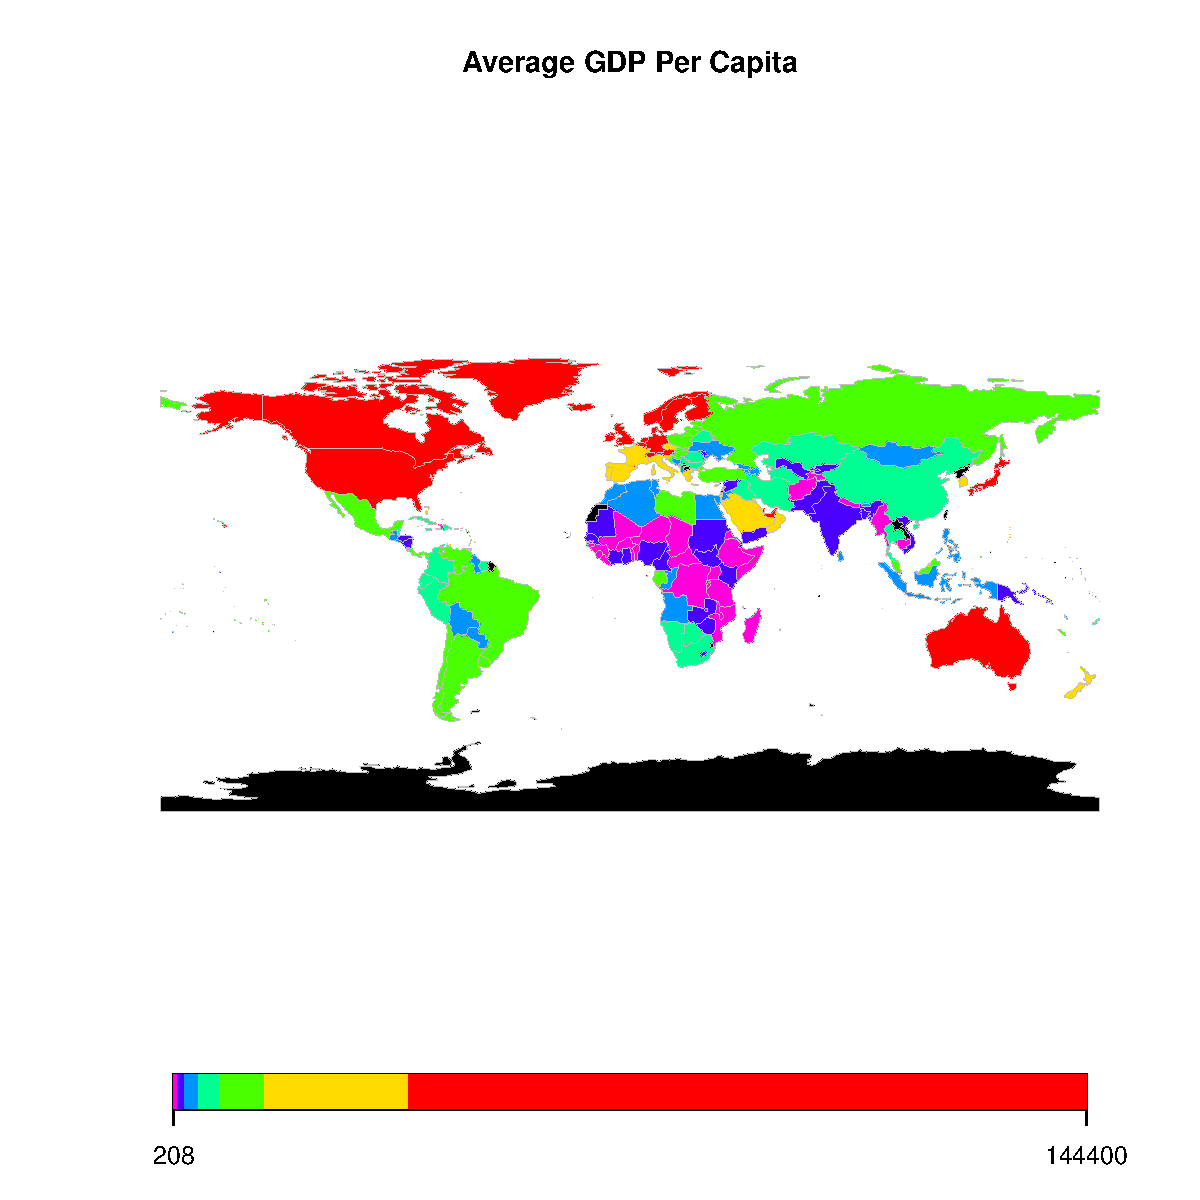
\includegraphics[width=\maxwidth]{figure/unnamed-chunk-20-1} 
\end{knitrout}
\caption{Map Representing Average GDP per capita}

\label{fig}
\end{figure}


\newpage
\subsection{Average Internet Users Percentage Map}
\begin{lstlisting}
average_internet_users<- world_bank_data %>%
  group_by(Country) %>%
  summarise(Internet_Users_Percentage = mean(Internet_Users_Percentage, na.rm = TRUE))


IUP <- joinCountryData2Map(average_internet_users, joinCode = "NAME", nameJoinColumn = "Country")


IUP_map <- mapCountryData(IUP, nameColumnToPlot = "Internet_Users_Percentage", mapTitle = "Average Internet Users Percentage", 
                           colourPalette = "terrain", missingCountryCol = "black")


\end{lstlisting}
This map shows the average GDP per capita of countries around the world. The countries with the lowest average internet users are in gray, the countries with moderate internet users are in orange and yellow  the countries with the highest average internet users are in green.The country without any data is represented in black.
\newpage
\begin{figure}[h!]
\centering
\begin{knitrout}
\definecolor{shadecolor}{rgb}{0.969, 0.969, 0.969}\color{fgcolor}\begin{kframe}
\begin{verbatim}
## 204 codes from your data successfully matched countries in the map
## 7 codes from your data failed to match with a country code in the map
## 39 codes from the map weren't represented in your data
\end{verbatim}
\end{kframe}
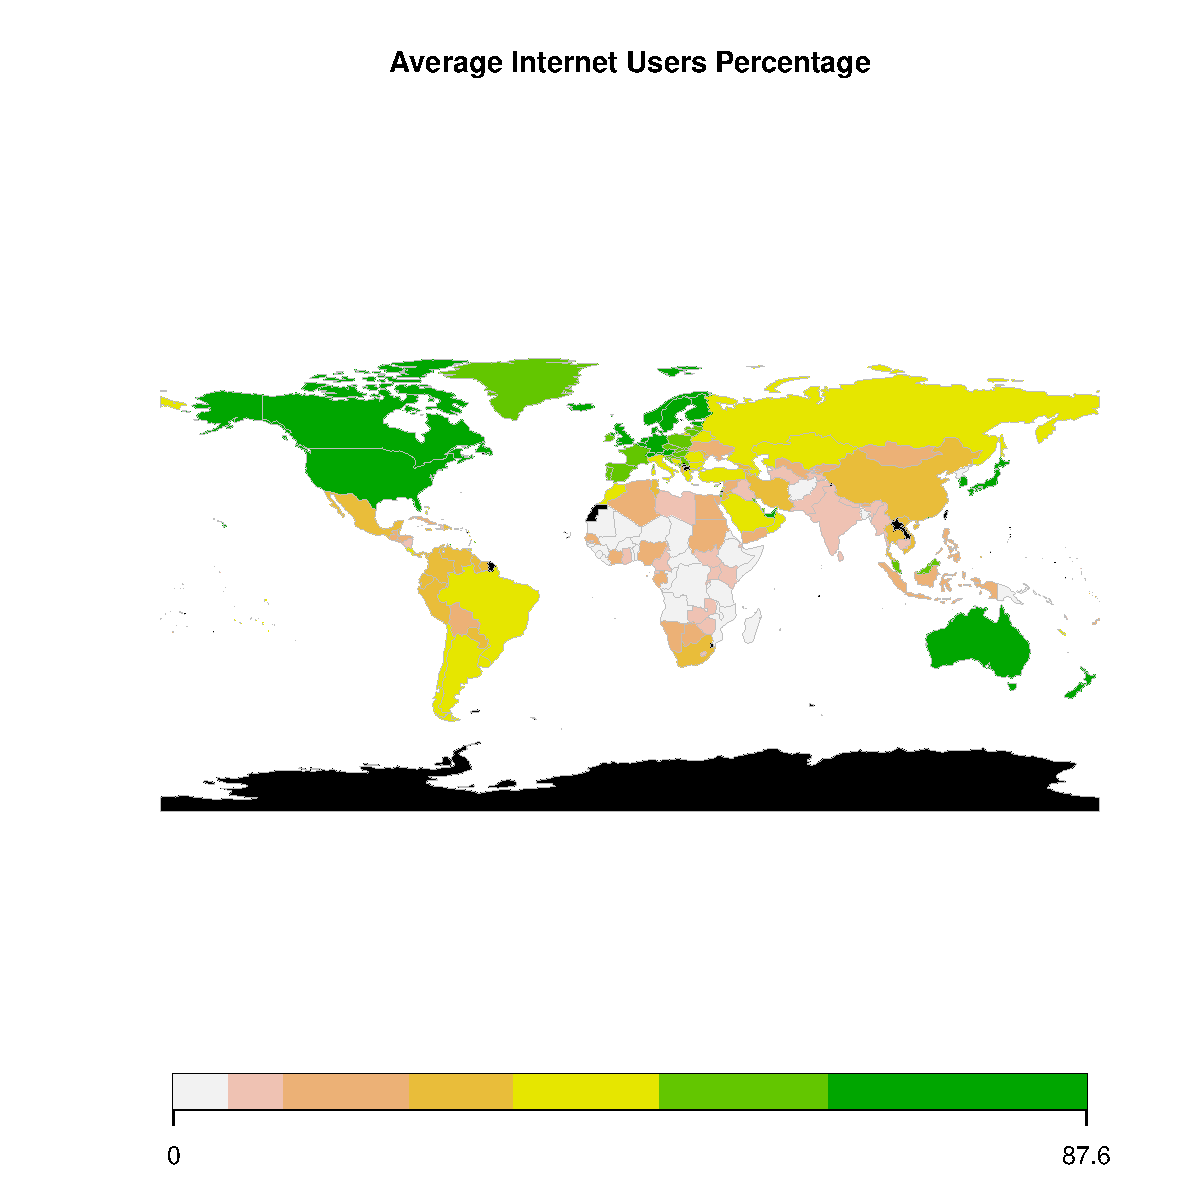
\includegraphics[width=\maxwidth]{figure/unnamed-chunk-21-1} 
\end{knitrout}
\caption{Map Representing Internet Users Percentage}

\label{fig}
\end{figure}


\newpage
\subsection{Average Infant Mortality Rate}
\begin{lstlisting}
average_Infant_Mortality_Rate<- world_bank_data %>%
  group_by(Country) %>%
  summarise(Infant_Mortality_Rate = mean(Infant_Mortality_Rate, na.rm = TRUE))


IMR <- joinCountryData2Map(average_Infant_Mortality_Rate, joinCode = "NAME", nameJoinColumn = "Country")


IMR_map <- mapCountryData(IMR, nameColumnToPlot = "Infant_Mortality_Rate", mapTitle = "Average Infant Mortality Rate", 
                          colourPalette = "white2Black", missingCountryCol = "white")


\end{lstlisting}
This map visualizes the average Infant Mortality Rate per country from 2000 to 2018. The color scale at the bottom indicates the birth rate, with grayish color representing lower Infant Mortality Rate and darker colors representing higher Infant Mortality Rate.The country without any data is represented in white.
\newpage
\begin{figure}[h!]
\centering
\begin{knitrout}
\definecolor{shadecolor}{rgb}{0.969, 0.969, 0.969}\color{fgcolor}\begin{kframe}
\begin{verbatim}
## 204 codes from your data successfully matched countries in the map
## 7 codes from your data failed to match with a country code in the map
## 39 codes from the map weren't represented in your data
\end{verbatim}
\end{kframe}
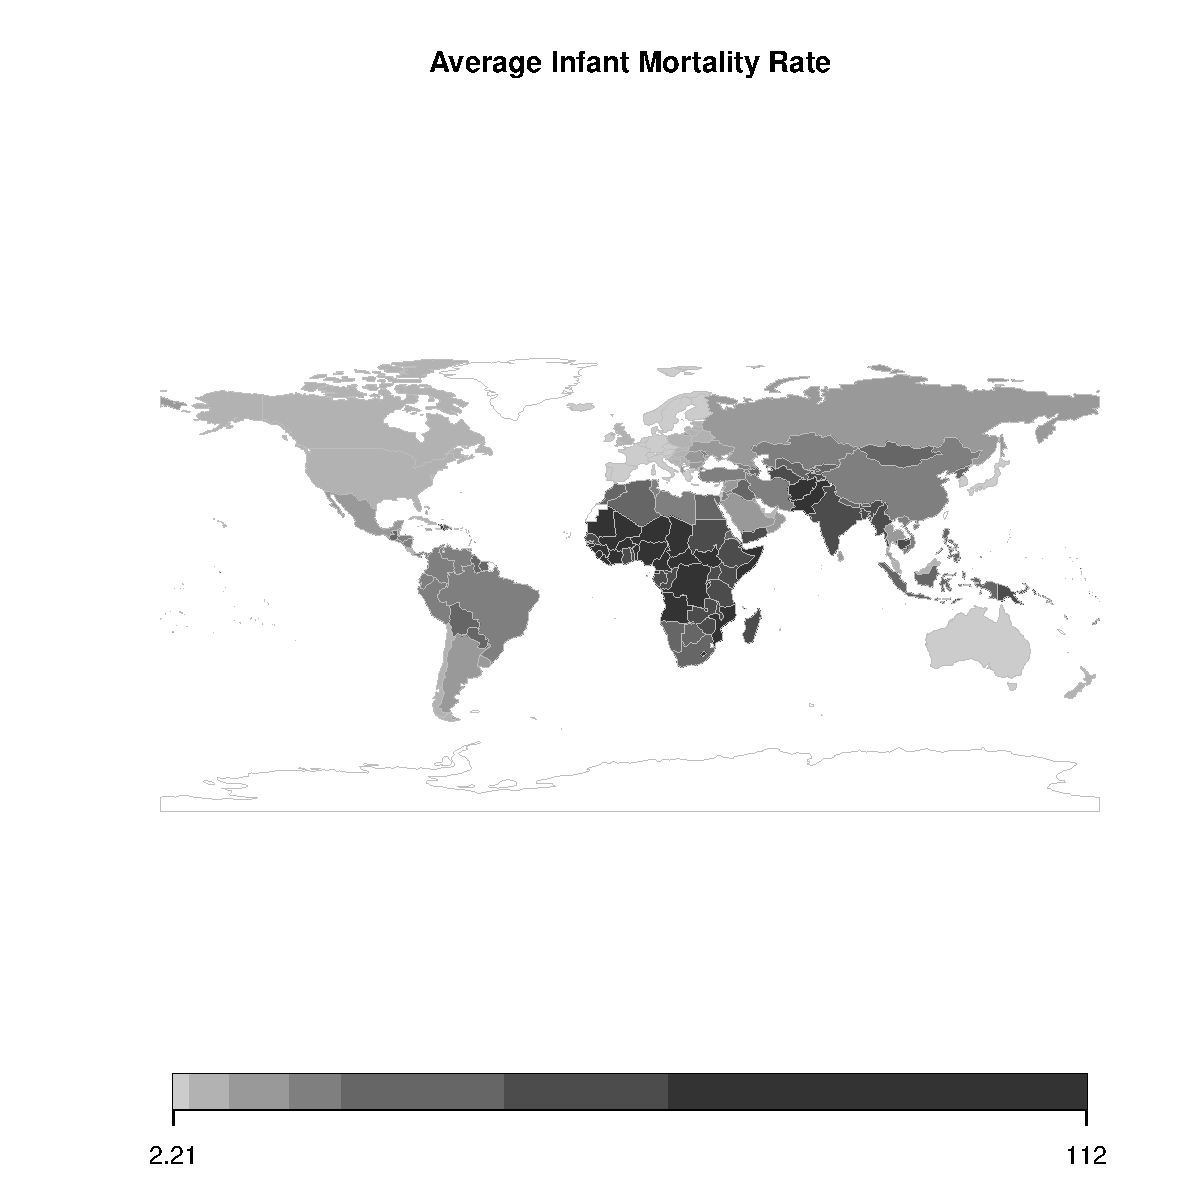
\includegraphics[width=\maxwidth]{figure/unnamed-chunk-22-1} 
\end{knitrout}
\caption{Map Representing Infant Mortality Rate}

\label{fig}
\end{figure}


\newpage
\subsection{Average Life Expentancy Map}
\begin{lstlisting}
my_palette <- brewer.pal(5, "Blues")

average_Life_Expentancy <- world_bank_data %>%
  group_by(Country) %>%
  summarise(Life_Expectancy = mean(Life_Expectancy, na.rm = TRUE))

LE <- joinCountryData2Map(average_Life_Expentancy, joinCode = "NAME", nameJoinColumn = "Country")

LE_map <- mapCountryData(LE, nameColumnToPlot = "Life_Expectancy", mapTitle = "Average Life Expectancy", 
                         colourPalette = my_palette, missingCountryCol = "black")


\end{lstlisting}
This map visualizes the average Life Expentancy Rate per country from 2000 to 2018. The color scale at the bottom indicates the birth rate, with grayish blue  color representing lower Infant Mortality Rate and darker blue color representing higher Infant Mortality Rate.The country without any data is represented in black.
\newpage
\begin{figure}[h!]
\centering
\begin{knitrout}
\definecolor{shadecolor}{rgb}{0.969, 0.969, 0.969}\color{fgcolor}\begin{kframe}
\begin{verbatim}
## 204 codes from your data successfully matched countries in the map
## 7 codes from your data failed to match with a country code in the map
## 39 codes from the map weren't represented in your data
\end{verbatim}
\end{kframe}
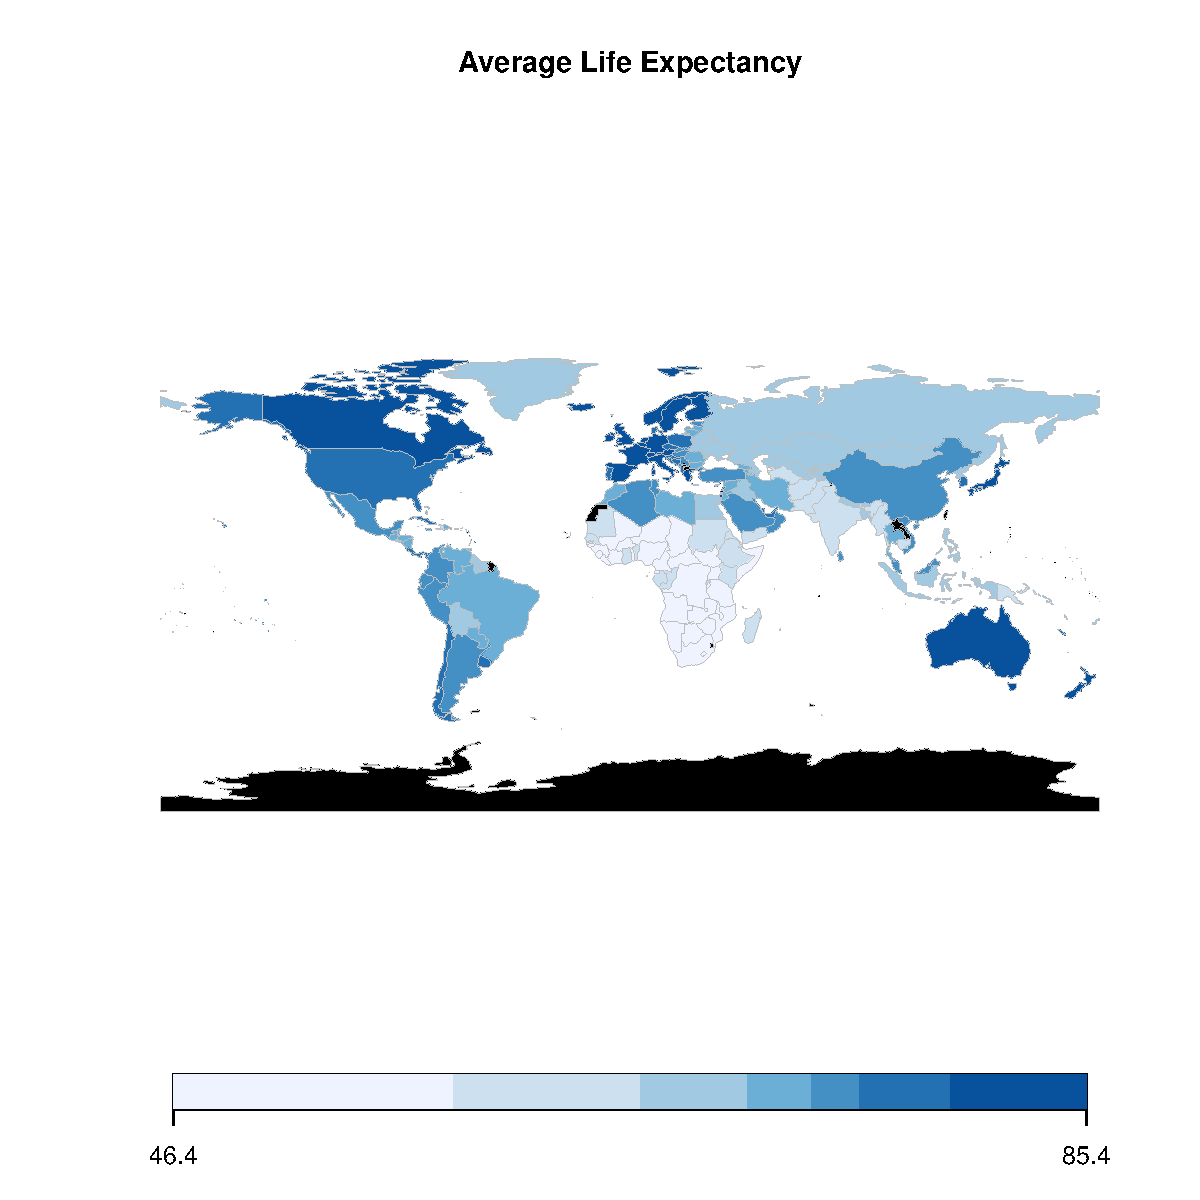
\includegraphics[width=\maxwidth]{figure/unnamed-chunk-23-1} 
\end{knitrout}
\caption{Map Representing Average Life Expentancy}

\label{fig}
\end{figure}



\newpage

\subsection{Average Population Density Map}
\begin{lstlisting}
my_palette2 <- brewer.pal(5, "Purples")

average_Population_Density <- world_bank_data %>%
  group_by(Country) %>%
  summarise(Population_Density = mean(Population_Density, na.rm = TRUE))

PD <- joinCountryData2Map(average_Population_Density, joinCode = "NAME", nameJoinColumn = "Country")

PD_map <- mapCountryData(PD, nameColumnToPlot = "Population_Density", mapTitle = "Average Population Density", 
                         colourPalette = my_palette2, missingCountryCol = "white")

\end{lstlisting}
This map visualizes the average Population Density Rate per country from 2000 to 2018. The color scale at the bottom indicates the Population Density, with lighter purple color representing lower population density Rate and darker purple color representing higher Population Density Rate.South Asia have the high population density among other region. The country without any data is represented in black.

\newpage
\begin{figure}[h!]
\centering
\begin{knitrout}
\definecolor{shadecolor}{rgb}{0.969, 0.969, 0.969}\color{fgcolor}\begin{kframe}
\begin{verbatim}
## 204 codes from your data successfully matched countries in the map
## 7 codes from your data failed to match with a country code in the map
## 39 codes from the map weren't represented in your data
\end{verbatim}
\end{kframe}
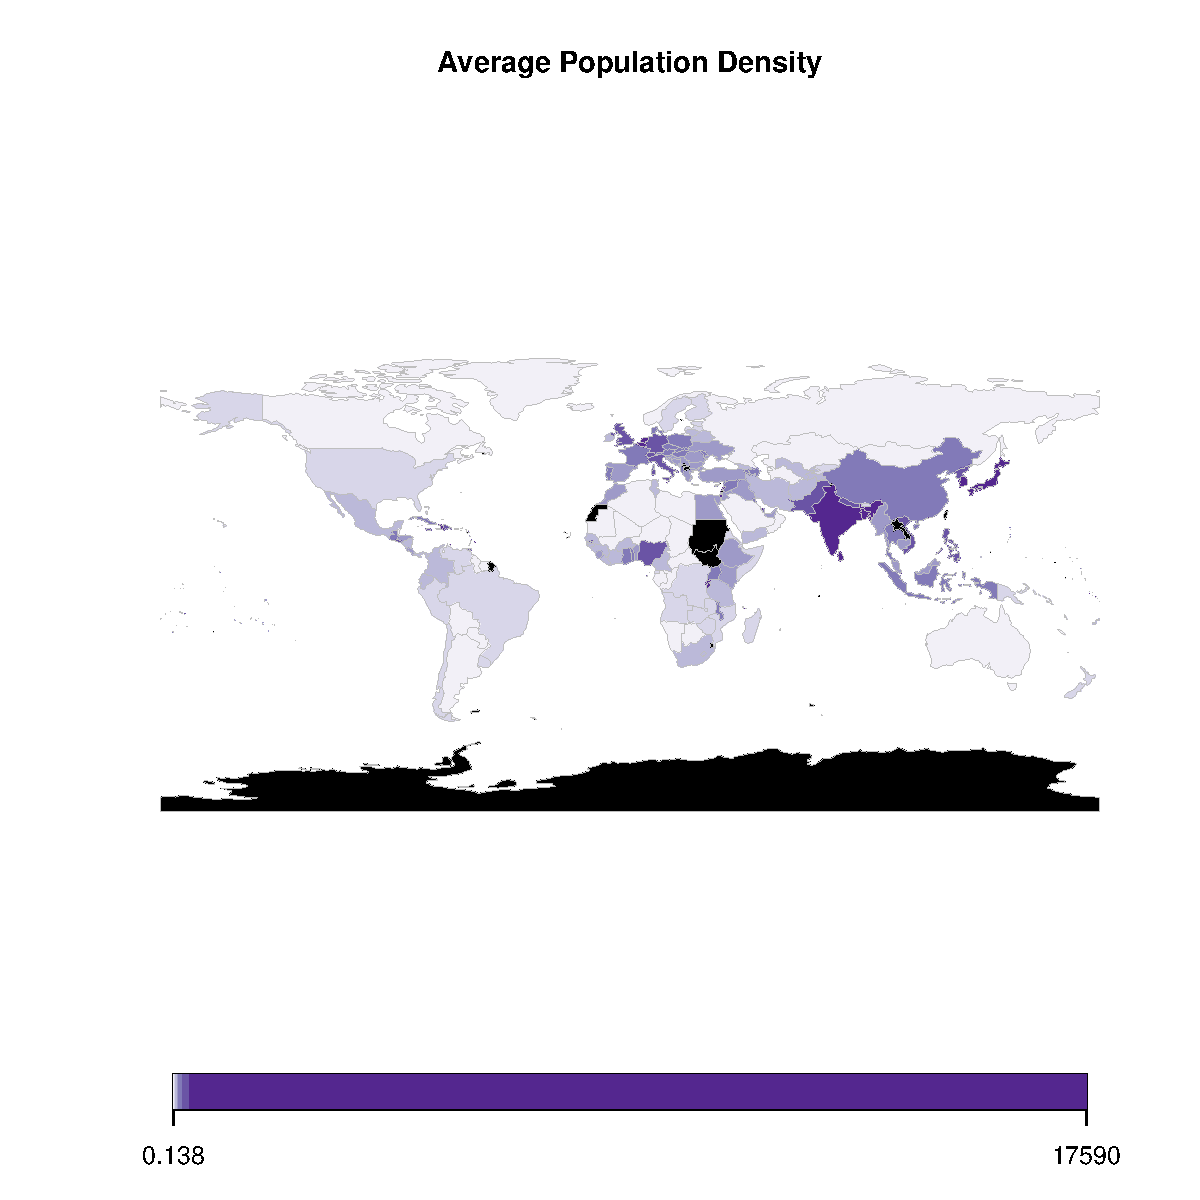
\includegraphics[width=\maxwidth]{figure/unnamed-chunk-24-1} 
\end{knitrout}
\caption{Map Representing Average Population Density}

\label{fig}
\end{figure}

\newpage
\subsection{Average Unemployment Rate Map}
\begin{lstlisting}
my_palette3 <- brewer.pal(5, "PuOr")

average_Unemployment_Rate <- world_bank_data %>%
  group_by(Country) %>%
  summarise(Unemployment_Rate = mean(Unemployment_Rate, na.rm = TRUE))

UR <- joinCountryData2Map(average_Unemployment_Rate, joinCode = "NAME", nameJoinColumn = "Country")

UR_map <- mapCountryData(UR, nameColumnToPlot = "Unemployment_Rate", mapTitle = "Average Unemployment Rate of Labour Force", 
                         colourPalette = my_palette3, missingCountryCol = "white")


\end{lstlisting}
This map visualizes the average Unemployment Rate of Labour Force per country from 2000 to 2018. The color scale at the bottom indicates the Population Density, with Orange color representing lower Unemployment Rate and purple color representing higher Unemployment Rate.South Asia have the low unemployment rate likely due to foreign Employment. The country without any data is represented in black.
\newpage
\begin{figure}[h!]
\centering
\begin{knitrout}
\definecolor{shadecolor}{rgb}{0.969, 0.969, 0.969}\color{fgcolor}\begin{kframe}
\begin{verbatim}
## 204 codes from your data successfully matched countries in the map
## 7 codes from your data failed to match with a country code in the map
## 39 codes from the map weren't represented in your data
\end{verbatim}
\end{kframe}
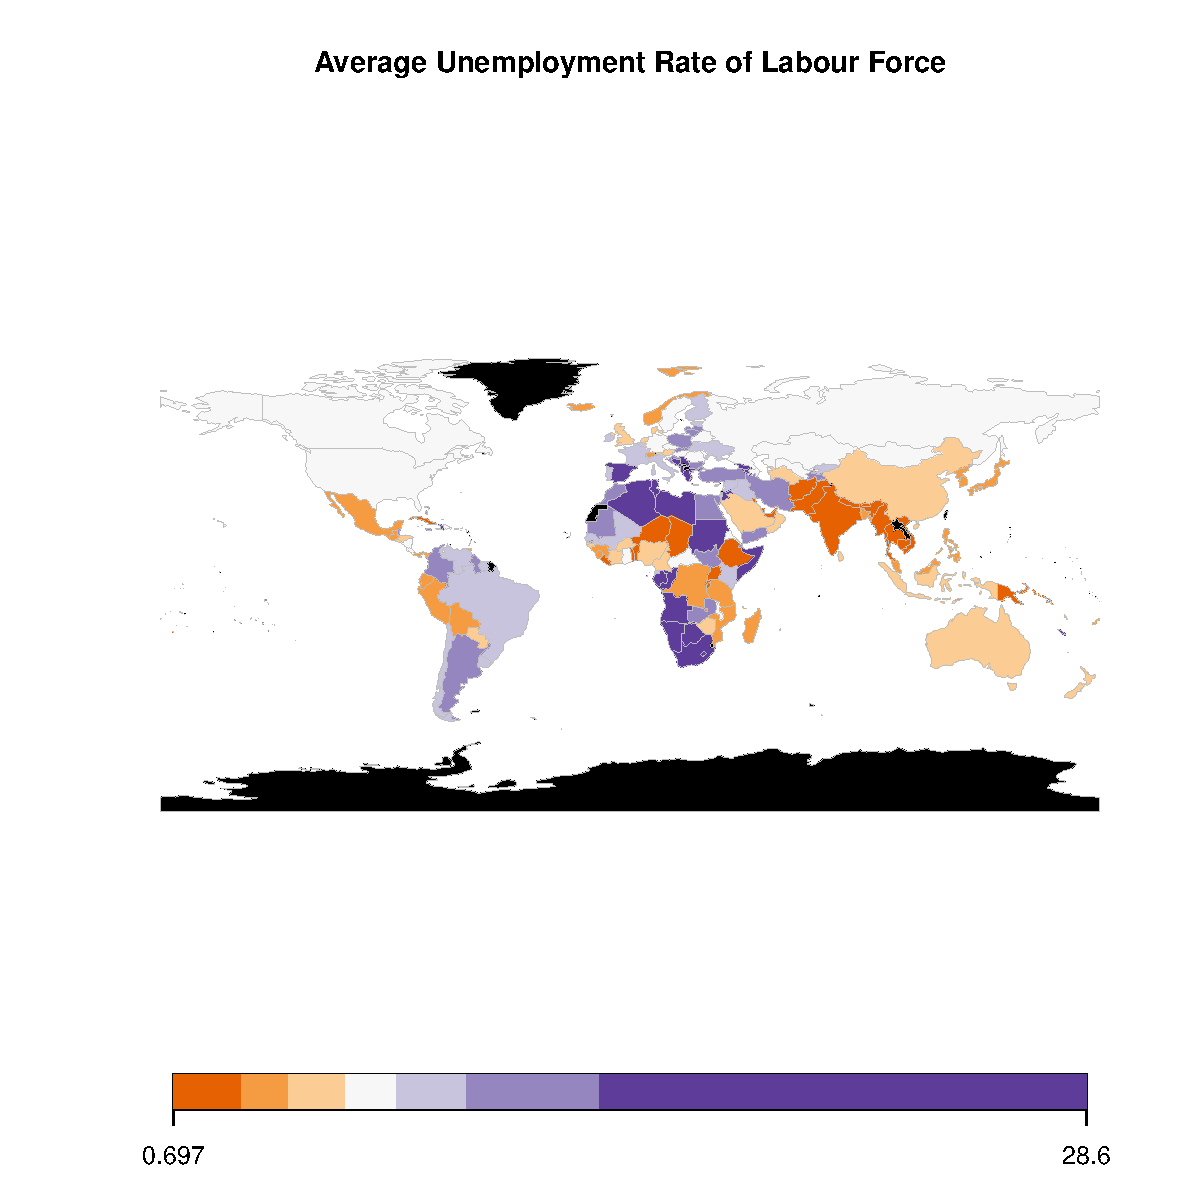
\includegraphics[width=\maxwidth]{figure/unnamed-chunk-25-1} 
\end{knitrout}
\caption{Map Representing Average Unemployment Rate}

\label{fig}
\end{figure}

\newpage
\section{Summary and Insights}
Using data from the World Bank, this paper investigated socioeconomic and demographic trends at the regional and national levels between 2000 and 2018. We discovered the data included life expectancy, GDP per capita, infant mortality, birth, and death rates, as well as population density, internet usage, and per capita electric power consumption. The findings suggest a range of correlations and trends derived from different global growth patterns:

\subsection{Answering Non-Trivial Questions}
\textbf{Trend Analysis and Comparisons}

\begin{enumerate}
    \item How have unemployment rates evolved across different regions and income groups?

    The unemployment rates have evolved differently across regions and income groups. Some regions have seen a decrease in unemployment rates, while others have seen an increase. For example, in East Asia and the Pacific, unemployment rates for all income groups have decreased since 2000. However, in Latin America and the Caribbean, unemployment rates have increased for all income groups since 2000. In general, high-income countries have lower unemployment rates than low-income countries.
    
    \item Does the relationship between life expectancy and GDP per capita vary across regions and income groups?
    
    Yes, the relationship between life expectancy and GDP per capita varies across regions and income groups. In general, there is a positive correlation between these two variables, meaning that countries with higher GDP per capita tend to have longer life expectancies. However, the strength of this relationship varies across regions and income groups. For example, in Sub-Saharan Africa, the relationship between life expectancy and GDP per capita is weaker than in other regions. This is likely due to a number of factors, such as the prevalence of infectious diseases, limited access to healthcare, and high levels of poverty. Additionally, the relationship between life expectancy and GDP per capita is also weaker for low-income countries than for high-income countries. 
    
    \item{What is the trend of Life Expectancy in region with different population Density?}
   
    The trend shows that, in general, countries with higher population density tend to have longer life expectancies than countries with lower population density. However, there are some exceptions to this trend. For example, South Asia  has a relatively high population density but also has a relatively low life expectancy. 
    
    \item How has the infant mortality rate changed over time in different regions?
    
    There has positive trend of decreasing infant mortality rates across various regions between 2000 and 2018. While Sub-Saharan Africa initially had the highest rate, it experienced the most significant decline. South Asia, starting with the second highest rate, experienced a significant decline as well. Europe and Central Asia witnessed the second most significant decrease, starting from a relatively low rate in 2000. Meanwhile, Latin America and the Caribbean, the Middle East and North Africa, and North America all exhibited gradual declines, from lower starting points in 2000. This overall trend showcases global progress in reducing infant mortality.
    
    \item Are there differences in the rate of change in birth rates between regions or income groups?
    
    Yes, there are clear differences in the rate of change in birth rates between regions and income groups. High income regions (both OECD and non-OECD) have generally lower birth rates than other income groups and have experienced a significant decline in birth rates over time.
Lower and upper middle income regions have higher birth rates, but the distribution is wider and varies more across regions.Low-income regions have the highest birth rates, with a wider distribution, suggesting a greater diversity in birth rate trends within these regions.

    \item Is the relationship between income group and death rate consistent across regions?
    
    No, the relationship between income group and death rate is not consistent across regions. While generally high-income countries have lower death rates, this pattern is not uniform. For example, in East Asia and Pacific, the death rates for high-income countries (non-OECD) are more similar to those of lower middle-income countries. Similarly, in Europe and Central Asia, the death rates for high-income (OECD) countries are comparable to those in upper middle-income countries, suggesting that other factors besides income group play a significant role in determining death rates within certain regions.
    
    \item How do birth rates and infant mortality rates vary across different regions? Are there significant differences between regions?
    
    There is a clear relationship between birth rate and infant mortality rate, with significant differences across regions. Sub-Saharan Africa has the highest birth rate and infant mortality rate, while East Asia and Pacific and Europe and Central Asia have the lowest. Overall, regions with higher birth rates tend to have higher infant mortality rates.
\end{enumerate}

\textbf{Correlation and Relationships}

\begin{enumerate}
    \item Is there a strong correlation between internet usage and GDP per capita?
    
    Yes, there is a strong positive correlation between internet usage and GDP per capita. The scatter plot shows a clear upward trend, with countries having higher internet usage also generally having higher GDP per capita. The correlation coefficient of 0.679 further supports this observation, indicating a moderately strong positive relationship.
    
    \item What are the correlations among various socio-economic variables in the dataset?
    
    The correlation heatmap reveals several interesting relationships among the socio-economic variables in the dataset:
    
    \textbf{Strong Positive Correlations:}
  \begin{itemize}
\item{GDP per Capita and Life Expectancy: Higher GDP per capita is strongly associated with higher life expectancy.}
\item{GDP per Capita and Internet Users Percentage: Wealthier nations tend to have greater internet penetration.}
\item{Electric Power Consumption per Capita and GDP per Capita: Countries with higher economic output typically consume more electricity per person.}
\end{itemize}

\textbf{Strong Negative Correlations:}
  \begin{itemize}
\item{Infant Mortality Rate and Life Expectancy: As expected, higher infant mortality rates are linked to lower life expectancy.}
\item{Infant Mortality Rate and GDP per Capita: Wealthier countries tend to have lower infant mortality rates.}
\end{itemize}

\textbf{Weaker/Less Clear Correlations:}
  \begin{itemize}
\item{Unemployment Rate and Many Variables: The heatmap doesn't show consistently strong correlations between unemployment and other factors displayed. This suggests that the relationship between unemployment and these socio-economic indicators is more complex and likely influenced by other variables not shown in this heatmap.}
\end{itemize}
  
\end{enumerate}

\section{Future Works}
In future , we can use time series analysis when working with the World Bank dataset to find trends and patterns over time for important metrics like GDP, population density, and life expectancy. Composition, trend analysis, and forecasting with techniques like ARIMA or exponential smoothing may be used in this.Another option is predictive modeling, where one can create models to project future values based on past data and other relevant factors. For example, we may create models based on internet usage, income group, and other socioeconomic factors to forecast life expectancy or GDP growth rates. These evaluations can offer insightful information about the possible course of the growth of a country and development.\citep{siami2018comparison}\hfill \break

Using cluster analysis is an additional strategy that groups nations according to their indicators in order to find similarities or unique characteristics. This can be useful for forecasting development trajectories, recognizing outliers, and comprehending regional patterns. Furthermore, by examining correlations between various indicators, researchers and policymakers can better understand the factors that influence outcomes and the drivers of economic growth, health outcomes, and other important measures. By utilizing the geographical information contained in the dataset, geospatial analysis can be used to display spatial patterns, identify regional inequities, and draw attention to the particular development issues that each area faces. To further improve the depth of research, machine learning techniques such as regression and classification can provide complex models for comprehending and forecasting global indicators.\citep{wierzchon2018modern}

\section{Conculsion}
The World Bank data from 2000 to 2018 is analyzed in this study to present a complex picture of global development. Although there are encouraging trends, such as a decrease in infant mortality and an increase in life expectancy, there are still large differences between areas and socioeconomic classes.

The information shows that there is a significant relationship between GDP per capita and measures like internet usage and life expectancy. It also means that improving these aspects of society needs economic development. Regional variations, however, suggest that other important criteria, such access to education and health care, also matter significantly in addition to income.
The results highlight the importance of personalized development strategies that take into account the unique circumstances of various geographical areas. 

\bibliographystyle{agsm}
\bibliography{biblography.bib}
\end{document}

